\chapter{Spatial audio}

\begin{chapterabstract}
    This chapter serves as an introduction to spatial audio.
    Different approaches to representing spatial audio information are presented,
    and their suitability for 360\degree{} video applications is discussed.
    A more in-depth section on ambisonics follows, accompanied by a brief 
    foray into the mechanisms behind human spatial hearing.
\end{chapterabstract}

\section{Spatial audio representations}

There are three main approaches to representing spatial audio information -
channel-based audio, object-based audio and scene-based audio. \cite{ebu_sbo_hoa}\cite{mpeg_3d_article}\cite{sba_using_hoa}
Each with their own advantages and disadvantages for specific applications. Let me briefly introduce each paradigm. 

\subsection{Channel-based audio}
CBA content consists of a set of audio signals, each of them intended to feed a loudspeaker
at a specific position relative to the listener. \cite{mpeg_3d_article} 
It is extensively used for 3D sound in broadcasting and film \cite{ebu_sbo_hoa}\cite{mpeg_3d_article},
but it's core design is flawed in assuming a fixed speaker layout.
Reproducing channel based content on a speaker layout with a number of channels that is different to the one it was produced for
requires using sophisticated downmixing or upmixing algorithms which may result in loss of quality and spatial resolution. \cite{mpeg_3d_article}\cite{brinkman2015effect}
A study performed by researchers at the Delft University of Technology shows that Dolby Surround, which 
employs a downmixing technique \cite{dolby_digital} to playback surround audio on stereo headphones, 
showed significantly lower perceived ``overall presence" than even traditional stereo (not utilising HRTFs). \cite{hoekstra20133d}\cite{brinkman2015effect}
Furthermore, channel-based audio doesn't account for the possibility of speakers being positioned differently than the intended layout (an occurrence common in the real world),
which will inevitably alter the directionality of sounds and make the experience differ from the one intended by the content creator(s).

While CBA has been used extensively for delivering surround audio content in film and video games, it has a lot of constraints stemming 
from the assumption of a specific speaker count and layout made during the production stage. 
The most important constraint for VR applications is the difficulty in rotating the sound scene as a whole, 
which is required to keep the sound positions anchored in space while the listener's head may rotate.
While it can be done, the results are subpar at best, and result in ``\emph{a sound that goes in and out of focus
as the channels move into and out of particular speakers}" \cite[p.~45]{new_realities_in_audio}.

The other two spatial audio paradigms - OBA and SBA, don't share these flaws of CBA. \cite{ebu_sbo_hoa}\cite{system_for_oba}
Instead of relying on a specific speaker layout, they describe the audio scene independently of the playback hardware (the end user's speakers or headphones),
allowing playback on arbitrary loudspeaker setups while preserving spatial information and 
general audio quality better than CBA transformed using downmixing or upmixing techniques. \cite{system_for_oba}\cite{sba_using_hoa}

\subsection{Object-based audio}
OBA, which originated in game audio \cite{cambridge_imm_audio_review}, describes audio in a more general way. 
The content is represented as a virtual sound scene - a collection of sound sources called objects. \cite{ss_with_speakers_review}
An audio feed, as well as metadata, describing how the sound should be rendered, is assigned to each object. \cite{ss_with_speakers_review}\cite{cambridge_imm_audio_review}
This representation allows OBA content to be rendered on the end user's hardware, accounting for 
their specific (possibly non-standard \cite{oba_panner_patent}) speaker configuration,
as well as in the form of binaural audio, which will be described in more detail later. \cite{system_for_oba}\cite{cambridge_imm_audio_review}

OBA comes with it's own disadvantages - the main of which being the direct correlation
between the number of individual sound objects, the bandwidth required to transmit the OBA content, and decoding complexity. \cite{ebu_sbo_hoa}
There are however proposed solutions to lower the required bandwidth by employing object grouping techniques. \cite{breebaart2019spatial}

Object-based audio seems to be much better suited for VR applications than CBA.
It brings the ability to differentiate between individual audio objects 
and adjust their position relative to each other which is indispensable for VR games.
While the interactivity potential OBA brings is enticing, it is not as beneficial for noninteractive content, and
the increased bandwidth requirements are undesirable, especially for 360\degree{} video streaming scenarios.

\subsection{Scene-based audio}

While SBA still uses the concept of channels,
the channels play a very different role - instead of associating each channel with a specific speaker, as in CBA,
or with a specific sound object, as in OBA, the channels in SBA are combined to equally capture 
the sound coming from all directions. \cite{new_realities_in_audio}\cite{sba_using_hoa}\cite{cambridge_imm_audio_review}

Ambisonics is the underlying mathematical framework that makes SBA possible.
It is a surprisingly old approach 
initially described by Michael A. Gerzon in 1972 in his article ``Periphony: With-Height Sound Reproduction" \cite{gerzon1973periphony}.
Ambisonic content can easily be transformed to allow playback on any speaker arrangement, it is computationally viable to decode, encode,
and apply simple processing, such as rotating the sound scene,
in real time, and it's flexible in allowing to lower the required bandwidth at the cost of decreased spatial resolution. \cite{new_realities_in_audio}\cite{qualcomm_sba}
Ambisonics is in fact so powerful, and such a good fit for 360\degree{} video, that it gets a dedicated section.

\section{Ambisonics}

\subsection{M/S Stereo}

To understand how ambisonics make all of this possible, let's start with a simpler concept -
stereo audio, specifically it's Mid/Side representation.
When the term stereo is mentioned, most readers will probably associate it with X/Y encoding where the audio is encoded using a left and right channel.
This representation is natural for humans, because it closely resembles the way our hearing works, 
but mid/side (commonly shortened to M/S) encoding (\cite{ms_herre2004joint}) brings significant advantages compared to X/Y. 
It is very easily downmixed to mono, and gives the ability to widen or narrow the stereo image. \cite{new_realities_in_audio}

It's easiest to explain how M/S encoding works on a recording example.
To record M/S stereo one needs two microphones - one with a cardioid or omnidirectional pattern,
and a second microphone with a figure-eight pattern, positioned at a 90\degree{} angle relative to the first microphone. 
The first microphone captures sound from a wide area in front of the microphone or from all directions, this microphone will provide the mid channel signal.
A figure-eight pattern microphone captures sound predominantly in front and behind it,
so when rotated 90 degrees it will provide the necessary information for our side channel.
To get a stereo field, the side channel is duplicated and one of the copies is phase shifted 180\degree{}.
Let's refer to the phase shifted version as \emph{S-} and the original side channel as \emph{S+}.
The left channel can then be calculated as \emph{L = M + S+} and the right as \emph{R = M + S-}. 
In practice this means hard-panning
\footnote{In music production and audio mixing, hard-panning a channel means routing it exclusively to a single speaker.
    This approach was popular when stereo was first introduced, and can be heard, for example, on many The Beatles records.}
the \emph{S+} channel left, and hard-panning the \emph{S-} channel right.
Figure \ref{fig:ms_stereo} visualises the microphone setup and channel routing.
To get a mono version, one can just use the mid channel, and to widen or narrow the stereo image,
the relative volume of the side channel can be adjusted. \cite{ms_recording_basics}\cite{new_realities_in_audio}\cite{ambisonics_practical_theory}


\begin{figure}
    \begin{center}
        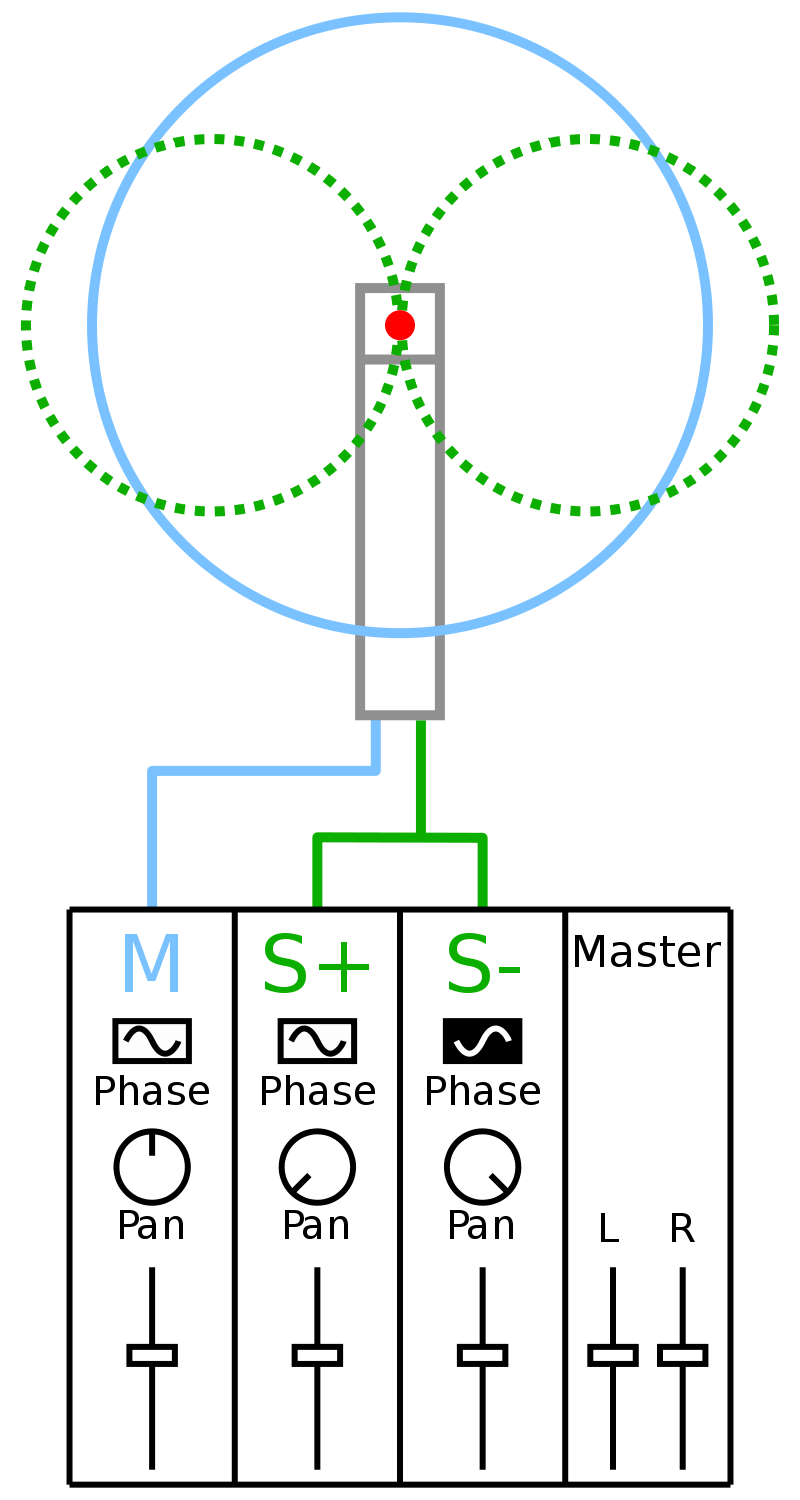
\includegraphics[height=20em]{images/spatial_audio/ms_stereo}       
        \caption{M/S stereo recording technique. Image sourced from \cite{recording_practices_wiki}. \label{fig:ms_stereo}}    
    \end{center}
\end{figure}

\subsection{From M/S stereo to B-format ambisonics}

The B-format is the minimal representation of ambisonics \cite{new_realities_in_audio}[p.~42]. It consists of four channels - 
\emph{W}, \emph{X}, \emph{Y} and \emph{Z}.
The role of the \emph{W} channel is analogous to the \emph{M} channel in M/S encoding - 
it captures sound coming from all directions equally. 
The other three channels - \emph{X}, \emph{Y} and \emph{Z} - are similar to the \emph{S} 
channel in M/S recording, but each one captures sound in a different plane,
the \emph{Y} channel - to the left and right of the listener, the \emph{X} channel - in front and behind,
and the \emph{Z} channel - above and below.
By distributing the source audio between the four channels, a sound can be positioned anywhere
on a sphere around the listener.
\cite{new_realities_in_audio}\cite{gerzon1973periphony}\cite{sba_using_hoa}

\subsection{Higher Order Ambisonics}
After the B-format was initially described, the mathematical framework
for ambisonics has been further extended, probably most notably by J{\'e}r{\^o}me 
Daniel when he described higher order ambisonics (HOA) in his Ph.D. thesis \cite{hoa_daniel}.
HOA extends the B-format by adding additional channels to increase the spatial resolution.
After the introduction of HOA, Gerzon's work was referred to as First Order Ambisonics.
To represent ambisonics of order \emph{N}, \emph{\((N+1)^2\)} channels are required.
Accuracy of the HOA representation of the original signal as well as localisation accuracy (spatial resolution) 
increase with increasing HOA order \emph{N}. \cite{ebu_sbo_hoa}\cite{new_realities_in_audio}

The next paragraphs will give a short summary of the mathematical apparatus behind higher order ambisonics.

\paragraph*{Functions defined on the surface of a sphere}
The following equation (\cite{rafaely_spherical_array_processing}) defines a spherical surface of unit radius in the Cartesian coordinate system:
\begin{equation}
        S^2 = \{\bm{x} \in \mathbb{R}^3: \lVert \bm{x} \rVert = 1\},
\end{equation}
where $\mathbb{R}^3$ is the three-dimensional space of real numbers, $\bm{x}$ represents a vector in
geometric notation, and $\lVert \bm{x} \rVert$ denotes the Euclidean norm (length) of the vector $\bm{x}$.
Any point on the surface of a sphere can be defined using spherical coordinates $(r, \theta, \phi)$; $r$ denotes the radius of the sphere, 
$\theta$ is the elevation angle, and $\phi$ is the azimuth angle.
Spherical functions are defined on the surface of a unit sphere (with $r=1$),
and accept the elevation and azimuth angles $\theta$ and $\phi$ as inputs. \cite{rafaely_spherical_array_processing}
An example spherical function can be seen in the following equation:
\begin{equation}
    f(\theta, \phi) = sin(\theta)cos^2(\phi),\ (\theta, \phi) \in S^2.
\end{equation}

\paragraph*{Spherical harmonics}
Spherical harmonics are a special set of spherical functions.
Each spherical harmonic function $Y^m_n(\theta, \phi)$ is denoted by it's order $n \in \mathbb{N}$
and it's degree $m \in \mathbb{Z}$. A graphical representation can be seen in figure \ref{fig:spherical_harmonics}.
A linear combination of the spherical harmonic 
functions can be used to approximate any square-integrable spherical function.
If the order of the spherical harmonics used is not limited, the resulting infinite series will 
accurately represent the original function. \cite{ambi_practical_theory_infinite_series_approximation}
Of course, an infinite series is not applicable for practical computations. 
Instead, a linear combination of spherical harmonics up to a specific order $N$ is used.
The accuracy of such an approximation increases with the maximum order $N$. 

\begin{figure}
    \begin{center}
        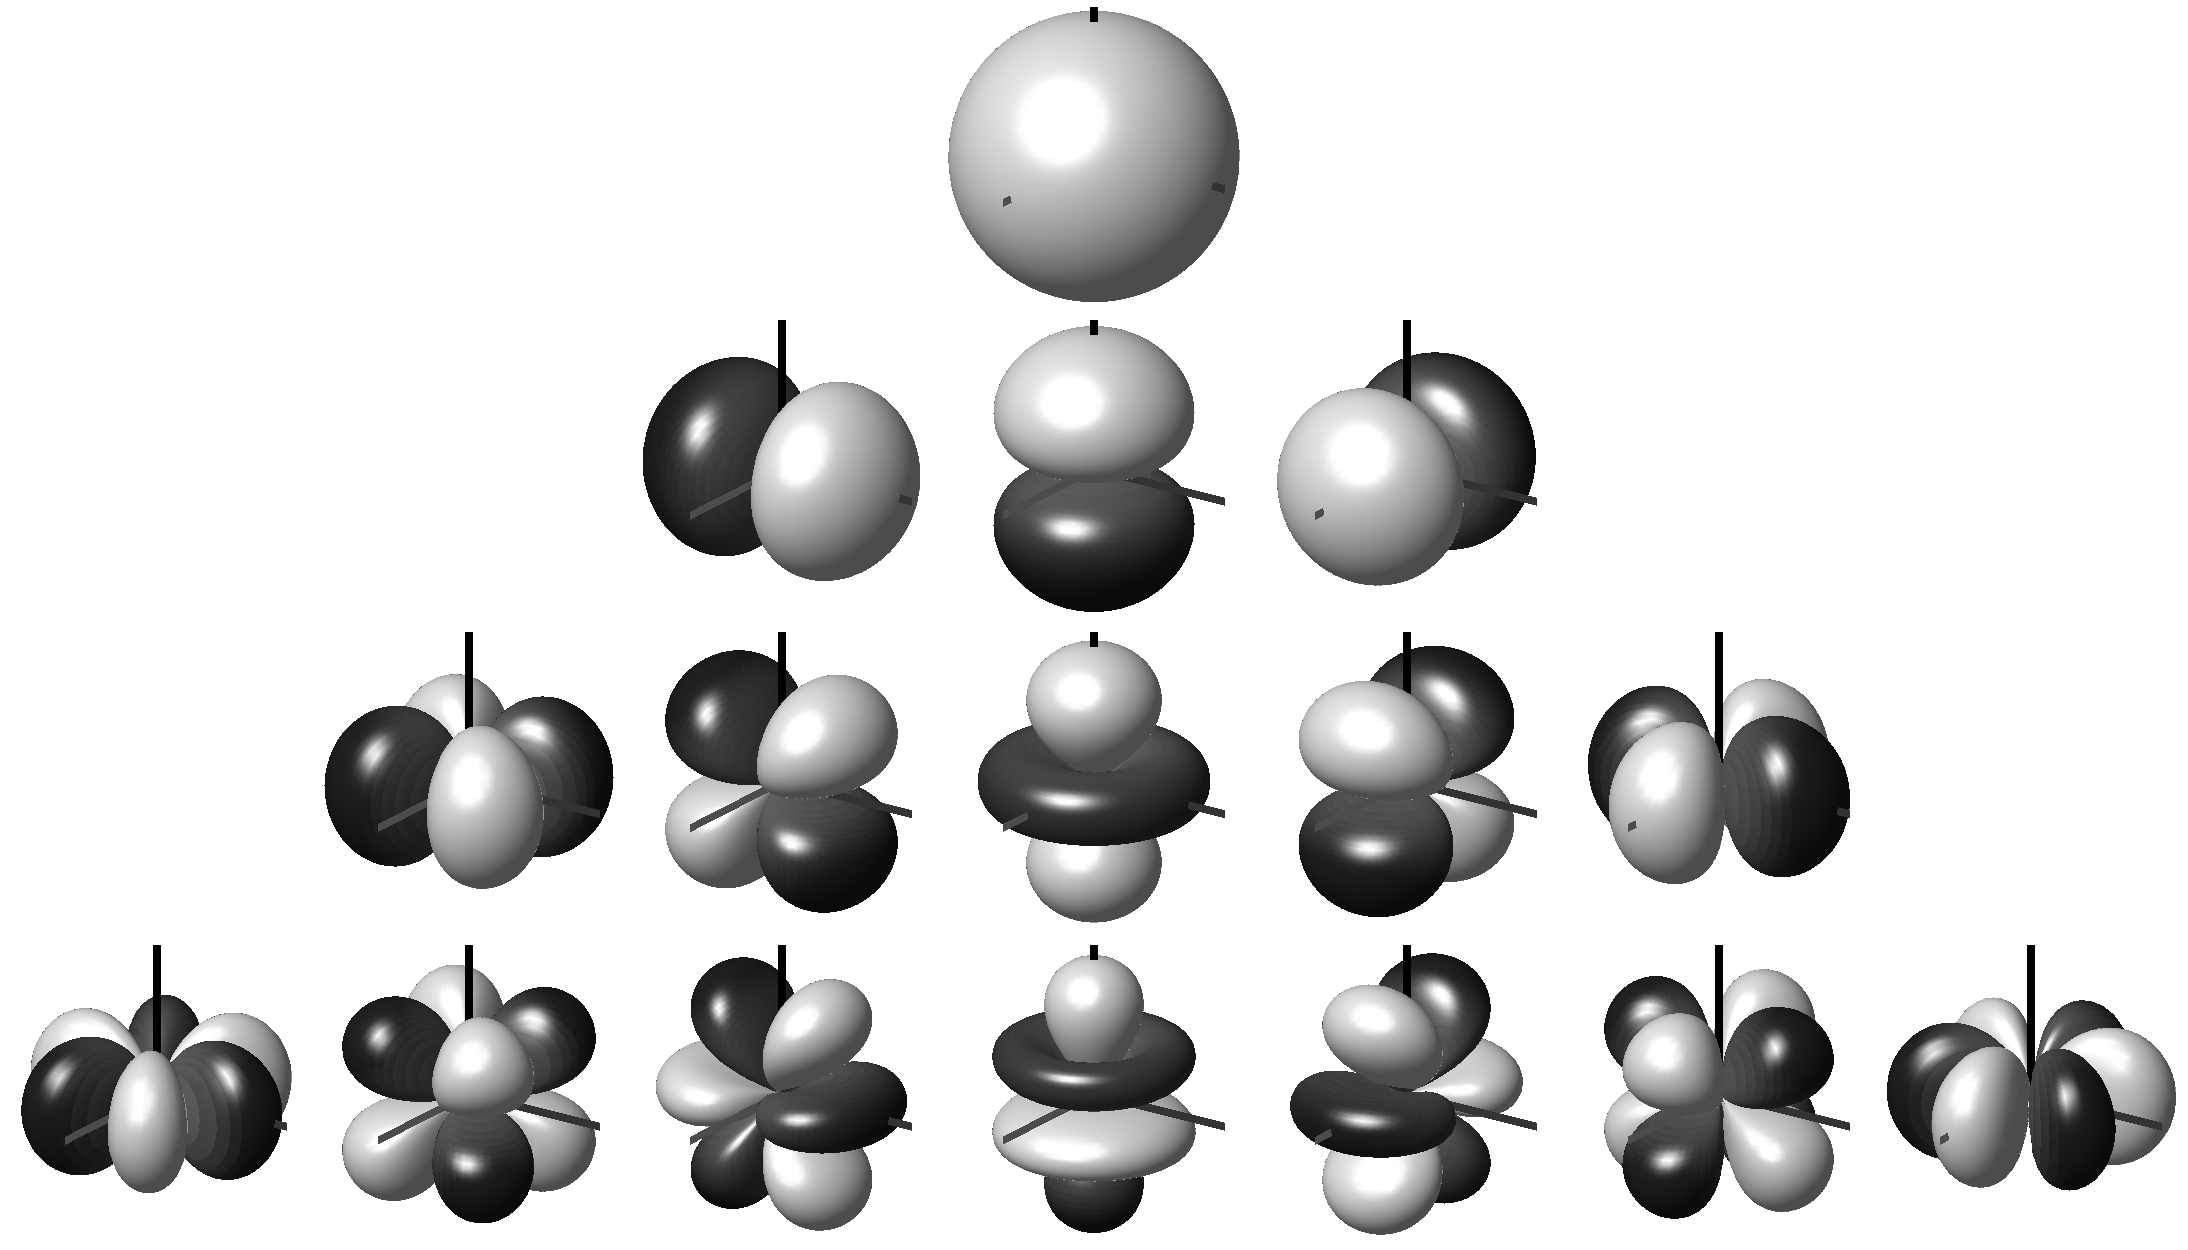
\includegraphics[height=20em]{images/spatial_audio/spherical_harmonics.png}       
        \caption{Balloon plots of spherical harmonics up to third order.
        The distance from the origin is defined by the absolute value of the given spherical harmonic.
        Dark portions represent negative values. (Order increasing towards the bottom of the picture; degree from left to right, with degree 0 in the middle.) 
        Image sourced from \cite{spherical_harm_pic_wiki}.\label{fig:spherical_harmonics}}
    \end{center}
\end{figure}

An ambisonics representation of a sound field is essentially ``a set of signals that would be obtained by microphones with specific directionality patterns'' 
(\cite{dickins_thesis}), and the spherical harmonic functions define the directionality patterns of these theoretical microphones. 
The values in the channels of an ambisonics-encoded audio signal 
are the coefficients used in the linear combination of spherical harmonics at a given time,
and the ambisonic order $N$ is equal to the maximum order of spherical harmonics used.
Returning to the M/S stereo example, it can be seen that the visualisations of first order spherical harmonics in figure \ref{fig:spherical_harmonics} 
closely resemble the figure-eight pattern of the microphone used
for the side channel. To gain a better intuitive understanding of ambisonic audio, 
higher order spherical harmonics can be thought of as representing increasingly complex microphone pickup patterns, 
and increasing the ambisonic order - as adding more microphones, with narrower patterns,
thus increasing the spatial resolution of the ambisonics representation.

Hopefully the brief summary presented above will provide 
the reader with a better intuitive understanding of how ambisonics make SBA a reality.
A more in-depth overview can be found in \cite{ambisonics_practical_theory} and
\cite{rafaely_spherical_array_processing}.

\subsection{Applying ambisonics in practice}

Ambisonics is a great theoretical framework for representing a sound scene, but, importantly, it is
also applicable in practice and brings many benefits during both the production and delivery stages.
Listed below, in no particular order, are some of the practical benefits ambisonics bring to the table:

\begin{itemize}
    \item Spatial audio content can be produced once, and decoded on the consumer's hardware.
    Because the decoding is performed on the end user's hardware, information about the playback environment, 
    such as the position and type of speakers, can be provided to the decoder. 
    With this information, a much better listening experience can be achieved than would otherwise be possible. \cite{ebu_sbo_hoa}\cite{new_realities_in_audio}\cite{qualcomm_sba}

    \item Ambisonics encoding, decoding, as well as rotation of the sound field can be performed very 
    fast\footnote{Especially if using SIMD compiler intrinsics (\cite{matmult_simd}\cite{intel_simd}\cite{arm_simd}) and other techniques employed by good mathematical libraries (e.g. \cite{high_perf_math_lib}).}
    on modern computers as most of the computation consists of matrix operations.
    Furthermore, when hardware resources are limited, computational power can be saved by rendering lower order ambisonics at the cost of fidelity
    - the extra HOA channels can just be discarded. \cite{ebu_sbo_hoa}

    \item Ambisonics content may sound even better years after it was initially produced. 
    Because ambisonics is such a general way to represent sound, in the future, advanced decoders can provide better sounding and more realistic 
    mixes than what is possible now. \cite{new_realities_in_audio}

    \item There are also multiple advantages to using Ambisonics as an intermediate spatial audio format in game engines. 
    Submixing is a very useful audio production technique. Essentially, it comes down to applying processing (audio effects)
    to multiple sounds at the same time. However, when submixing object based audio, the directionality of individual sounds can't be preserved
    - the whole submix has to become a single sound object. By submixing multiple sound objects into an ambisonics representation,
    the directionality of individual sounds can be preserved, while still allowing to process the submix as a whole.
    Utilising ambisonic submixes or even converting the whole mix to ambisonics
    before it gets rendered for playback can also bring performance advantages compared to processing each sound object individually.
    \cite{wwise_working_with_oba}\cite{wwise_ambisonics_intermediate_repr}
\end{itemize}

With these key advantages in mind it becomes obvious that ambisonics is a great fit for 360\degree{} video.
It should be no surprise that it is already being adopted for such applications. 
One example is the ability to upload 360\degree{} video with ambisonics audio to YouTube. \cite{youtube_ambisonics}
A big platform like YouTube supporting ambisonics and 360\degree{} video is a milestone in the adoption
of these technologies. It seems highly probable that user-created immersive content 
will increase in popularity in the coming years, as the availability of devices capable of 360\degree{}
video and audio recording increases. %//TODO: maybe mention apple's push into spatial audio

\section{From data to sound}

A detailed description of the inner workings of ambisonic decoding techniques is outside the scope of this thesis, 
but it wouldn't be complete without a brief overview of the existing approaches and the possibilities they bring in practice.
Ambisonics decoding is largely based on how humans perceive sound, so let's take a look at that in a bit more detail.

\subsection{Spatial hearing} \label{subsection:spatial_hearing}

Human hearing is fascinating - with just two points in space at which the sound field is sampled - our ears, 
we can tell the direction and distance to the sound source, if it's moving or not (and, roughly, at what speed), 
and many other things about the sound itself, as well as the surrounding environment.
In doing that, we rely on numerous acoustical cues that help us in locating the sound source,
but also, to a great extent, on our knowledge of the world - making assumptions based on previous experience. \cite{localization_clinical_neurology}\cite{auditory_distance}\cite{new_realities_in_audio}

Imagine you hear the sound of a helicopter flying in the distance, somewhere outside your field of view.
Based on the sound alone, you immediately assume numerous things about your surroundings:
\begin{itemize}
    \item You can tell that there's a helicopter flying because you know what a helicopter sounds like.
    \item You can roughly estimate how far away it is, because you know 
    how loud a helicopter is, and based on the ratio of environmental reflections (reverberations) to the pure sound
    - again, relying on previous experience of hearing a helicopter at a known distance.
    \item If you are in a city, surrounded by tall buildings, depending on the distance to the helicopter, your ability to localise the sound may be severely 
    impaired because the sound reaching your ears has been reflected multiple times by nearby buildings.
    \item If you are in a field, on the other hand, you should be able to estimate where it is quite precisely. 
\end{itemize}

Hopefully this shows how complex our perception of sound is, and puts to light some of the many factors - external and internal, that can affect it.
I must note that the above example is merely illustratory, not a description of a specific experiment.
It is however inspired by research in the field of auditory localisation.
A good overview of such research can be found in \cite{localization_clinical_neurology} and \cite{auditory_distance_moore}.

Let's now explore the problem of sound localisation from a more theoretical point of view.
It has long been suspected that our ability to detect the direction of sounds
stems from perceiving differences in the sound reaching each ear.
English physicist and baron, Lord Rayleigh, has determined through ingenious experiments, 
often involving tuning forks, that the perception of direction of sound is affected 
by differences in amplitude and phase of the sound waves between each ear. The article (\cite{on_our_perception_of_dir_of_sound}) describing his findings is dated April 3, 1876. 
His findings have later been confirmed with modern experiments. Nowadays we know of three main auditory cues instrumental in horizontal plane sound localisation - interaural loudness difference,
interaural time difference, and interaural phase difference.
While these are not the only factors at play, and it's impossible to say with any certainty that there aren't any we are still not aware of,
they are quite easily simulated, play a major role in auditory spatial perception,
and thus are very useful in spatial audio decoding.
\cite{localization_clinical_neurology}\cite{sound_localization_article}\cite{new_realities_in_audio}

\begin{itemize}
    \item Interaural intensity difference (IID) or interaural loudness difference (ILD) 
    is the loudness difference between the sound reaching each ear.
    A sound coming predominantly from one side, will be perceived as louder by the ear closest to it,
    as the head will partially block the sound before it reaches the other ear.

    \item Interaural time difference (ITD) is the difference between when a sound reaches each ear. 
    A sound directly in front of the listener would reach each ear at roughly the same time,
    while a sound to the listener's left would reach the left ear slightly before the right ear. 
    The human brain effortlessly notices these timing differences and interprets 
    them as information about the position of a sound source on a horizontal plane. 

    \item Interaural phase difference (IPD) is affected by the ITD and the frequencies a sound is composed of.
    A sine wave with a frequency of 1000 Hz that reaches one ear 0.5 ms before the other, will result in an IPD of 180\degree{}.
    Humans can detect IPDs as small as 3 degrees, but only for frequencies below 1000 to 1300 Hz. \cite{new_realities_in_audio} %//TODO: maybe not the best source
\end{itemize}

Interestingly, the effectiveness of these cues
varies depending on the sound's frequency composition. At lower frequencies sound
localisation mostly relies on ITDs and IPDs, while IIDs are important at higher frequencies. 
This can be explained by the fact that shorter (high frequency) waves are easily blocked by the listener's head,
while longer ones can reach the other ear with minimal amplitude degradation,
thus making IID cues inefficient at lower frequencies.
This again has been described by Lord Rayleigh in the 19th century, and has since been termed the ``duplex'' theory.
\cite{localization_clinical_neurology}\cite{on_our_perception_of_dir_of_sound}

\begin{figure}[!ht]
    \begin{center}
        \hspace{4em}
        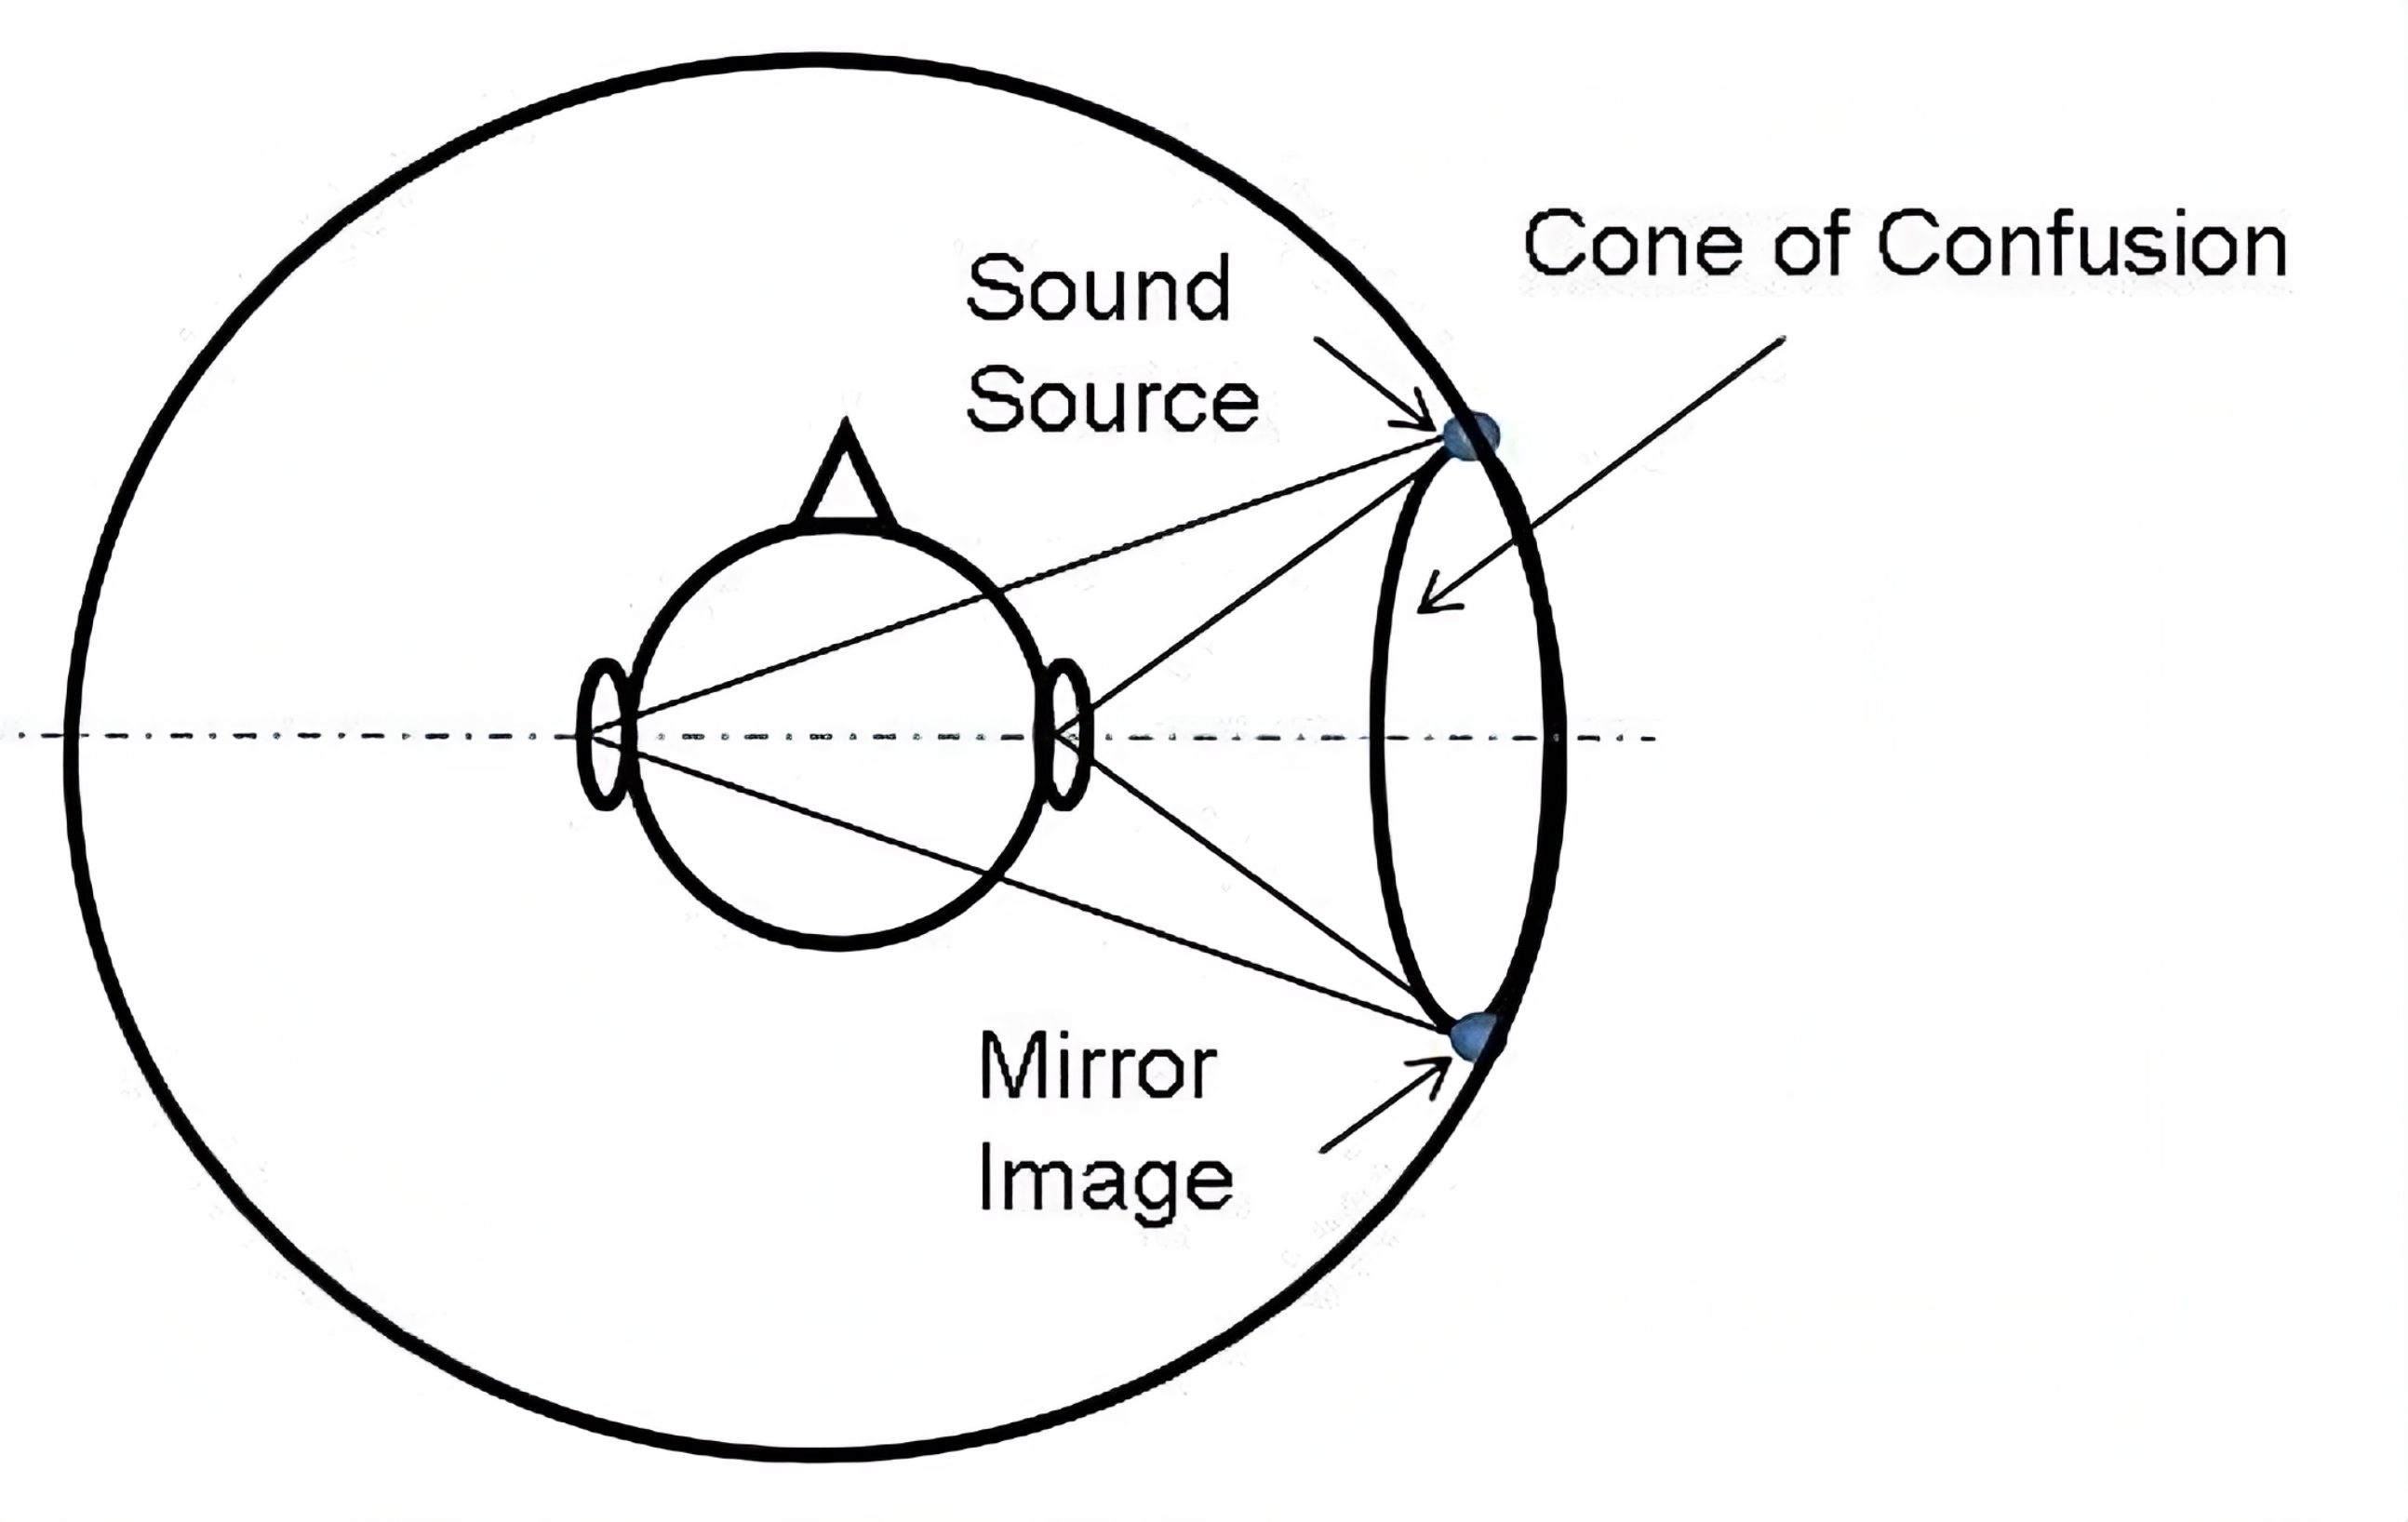
\includegraphics[height=10em]{images/human_hearing/cone_of_confusion.jpeg}       
        \caption{Cone of confusion. Image sourced from \cite{cone_of_conf_img_src}. \label{fig:cone_of_confusion}}    
    \end{center}
\end{figure}

The cone of confusion is another important concept in sound localisation research. 
As illustrated in figure \ref{fig:cone_of_confusion}, sounds located at specific points inside the so-called cone of 
confusion result in identical interaural timing, phase, and level differences. 
This makes interaural differences ineffective in discerning sounds in front and behind the listener, as well as above and below.
To alleviate this ambiguity, human listeners tend to move their head when trying to locate a sound.
Turning the head helps mitigate front/back confusion, and tilting the head aids vertical sound localisation.
For the same reason, many animals posses the ability to individually move each ear, removing the need for whole-head movement. \cite{new_realities_in_audio}
Vertical and front/back sound localisation is however still possible without head movement.
For sound having a relatively broad and flat spectrum, as is often the case in nature, 
direction-dependant filtering by the head and pinnae (the flaps on the outer ear)
provides vertical and front/back directional cues. \cite{localization_clinical_neurology}

The interaural difference and spectral filtering cues are helpful in detecting the direction of a sound,
but there is another dimension to our spatial hearing - distance.
Auditory distance perception is far less accurate than our ability to detect the direction to a source of sound. 
``\emph{The principal acoustic cues for distance perception are intensity (i.e., sound level arriving at the listener’s ears), 
direct-to-reverberant  (D/R)  energy  ratio,  and ILD. The relative importance of these cues varies widely across conditions.}" \cite{localization_clinical_neurology}
An in-depth discussion of these distance cues, and some other aspects of spatial hearing is outside the scope of this thesis, but I highly recommend 
Chapter 6 of \cite{localization_clinical_neurology} for further reading.

\subsection{Basic examples of ambisonic decoding}

\begin{figure}
    \centering
    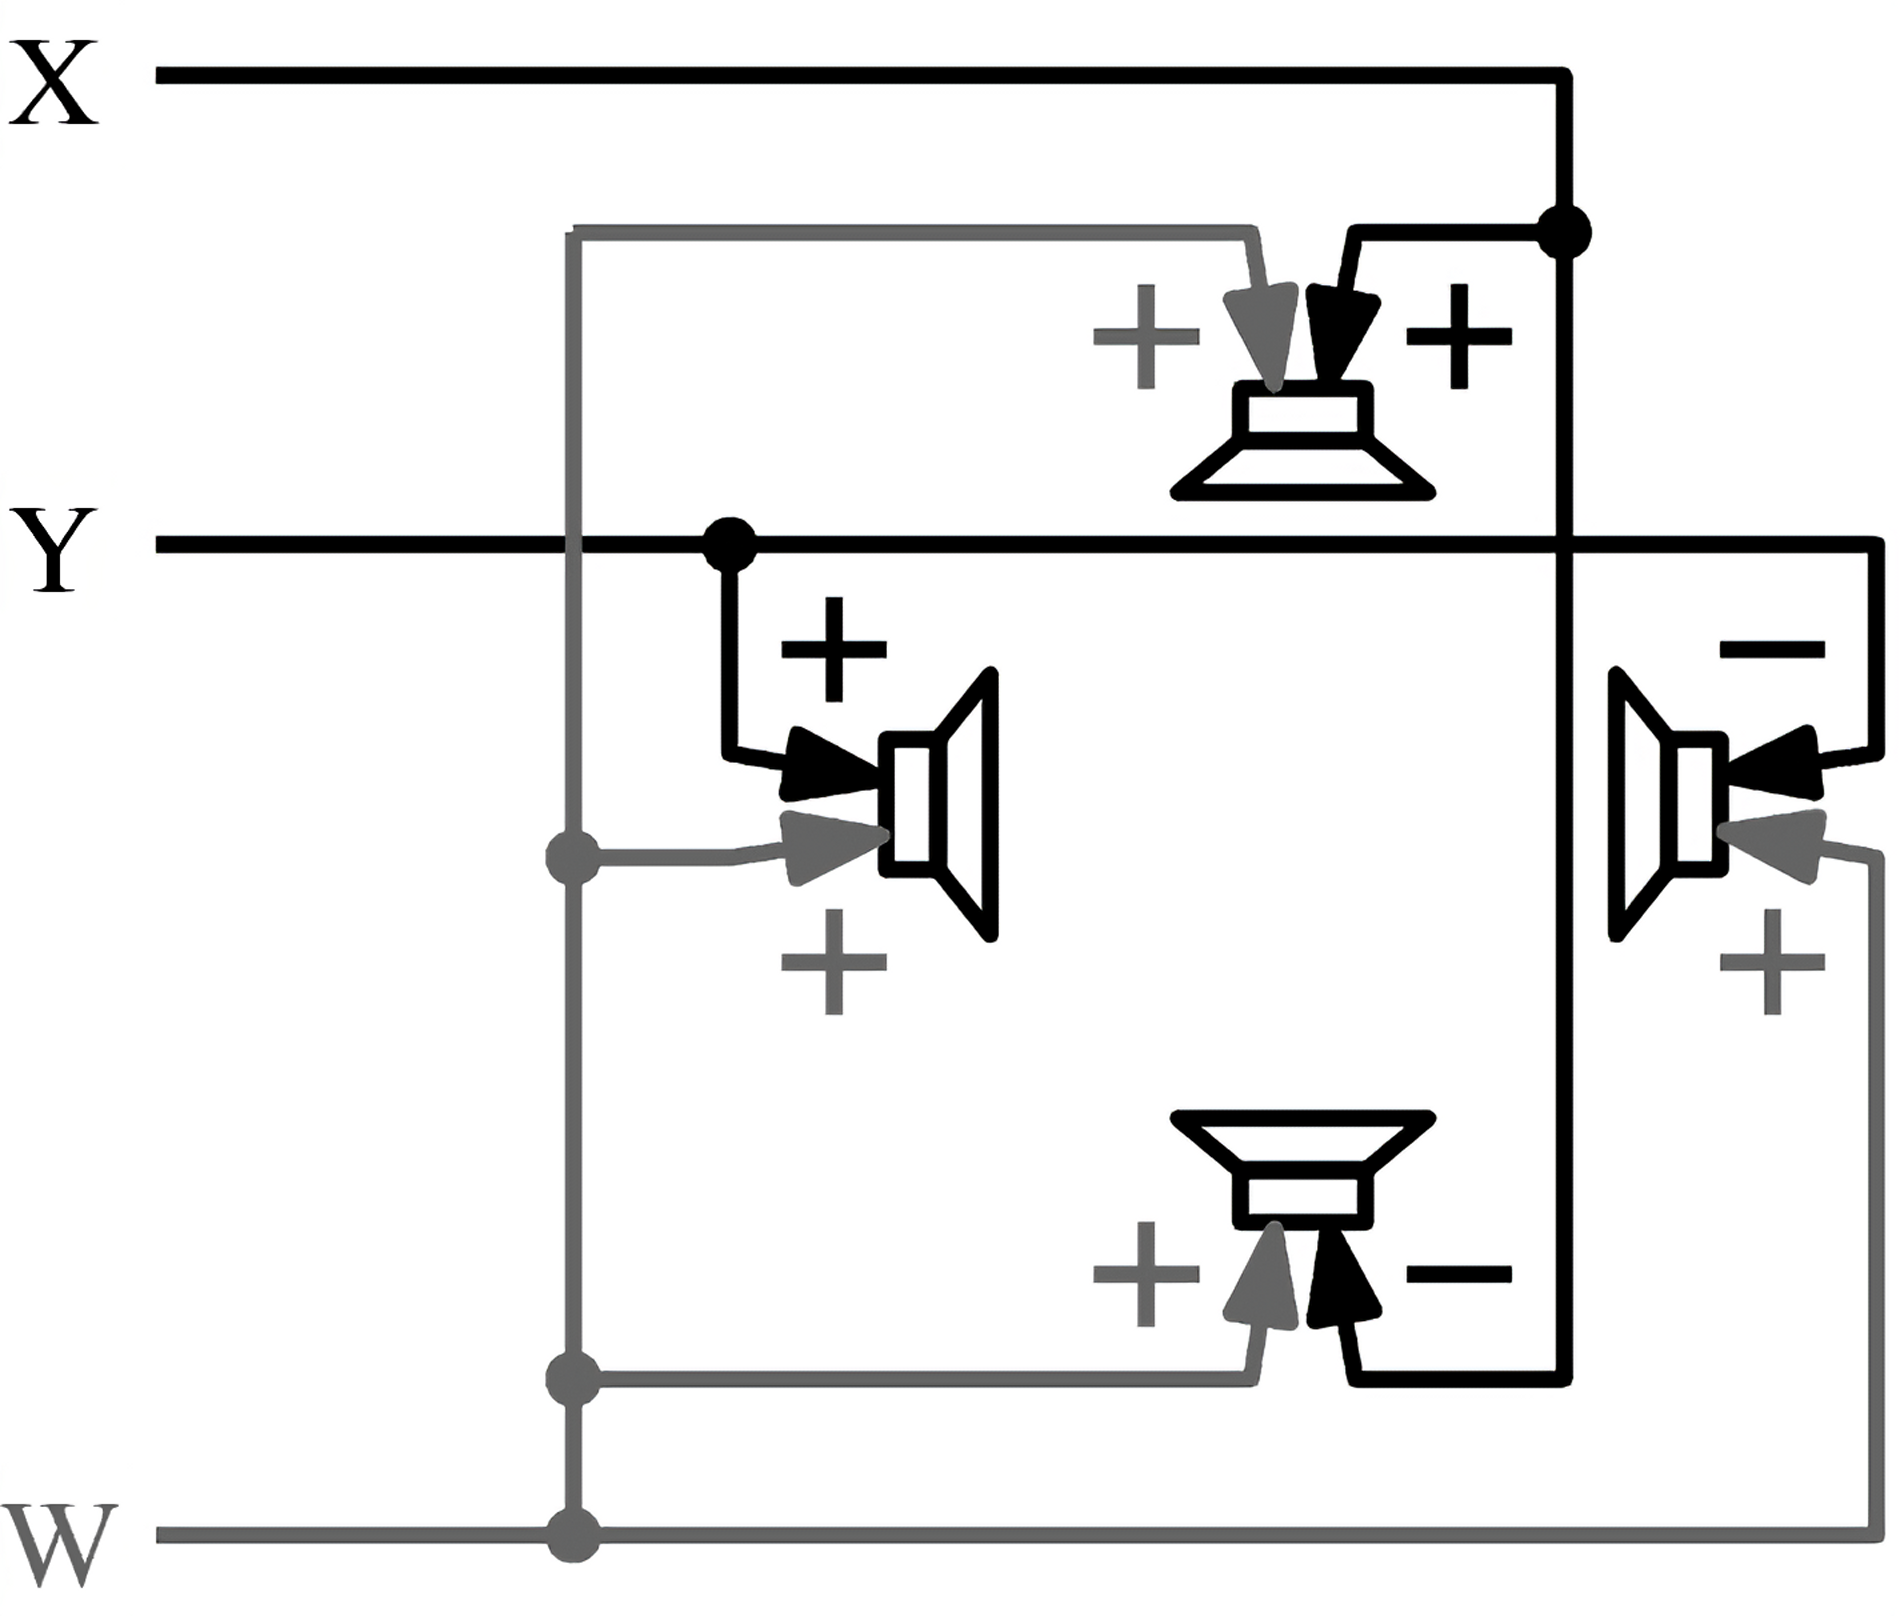
\includegraphics[height=10em]{images/spatial_audio/WXY_playback.png}       
    \caption{The \emph{WXY} channels routed to 4 speakers for 2D ambisonics playback
        Image sourced from \cite{ambisonics_practical_theory}.
        \label{fig:wxy_decoding}}
\end{figure}

Decoding ambisonics is the process of transitioning from the whole-scene representation 
back to separate channels that can be played back using individual speakers.
For the sake of simplicity let's first take a look at playing back 3 out of 4 B-format channels using 4 speakers. 
The only processing required for playback is adjusting the phase of the \emph{X} and \emph{Y} channels by 180\degree{} 
for the right and back speakers respectively as seen in \ref{fig:wxy_decoding}. 
(The front and left speaker receive the unadjusted signal from the \emph{X} and \emph{Y} channels, and all speakers receive the \emph{W} channel equally.)
It should be emphasized, that the Z channel is not utilised in this configuration, and thus height information is lost.
%TODO: more references

The previous example assumes an ideal loudspeaker layout. Unfortunately, that assumption almost never holds true in practice, 
and thus it is required to playback ambisonic audio with loudspeakers positioned at arbitrary angles towards the listener.
To achieve this, it is required to know the angle from each speaker to the listener. 
Figure \ref{fig:3d_sampling_decoder_equation} shows how this can be achieved in practice. 
$\Theta_1 ... \Theta_L$ are the direction vectors for the loudspeakers; 
$\Theta_X$, $\Theta_Y$ and $\Theta_Z$ are the unit vectors for the 
\emph{X}, \emph{Y} and \emph{Z} channels respectively. 
The speaker signals ($[S_1 ... S_L]$ are calculated by multiplying 
the source signal vector $[W X Y Z]^T$ with the decoding matrix $D$. \cite{ambisonics_practical_theory}

\begin{figure}[!ht]
    \centering
    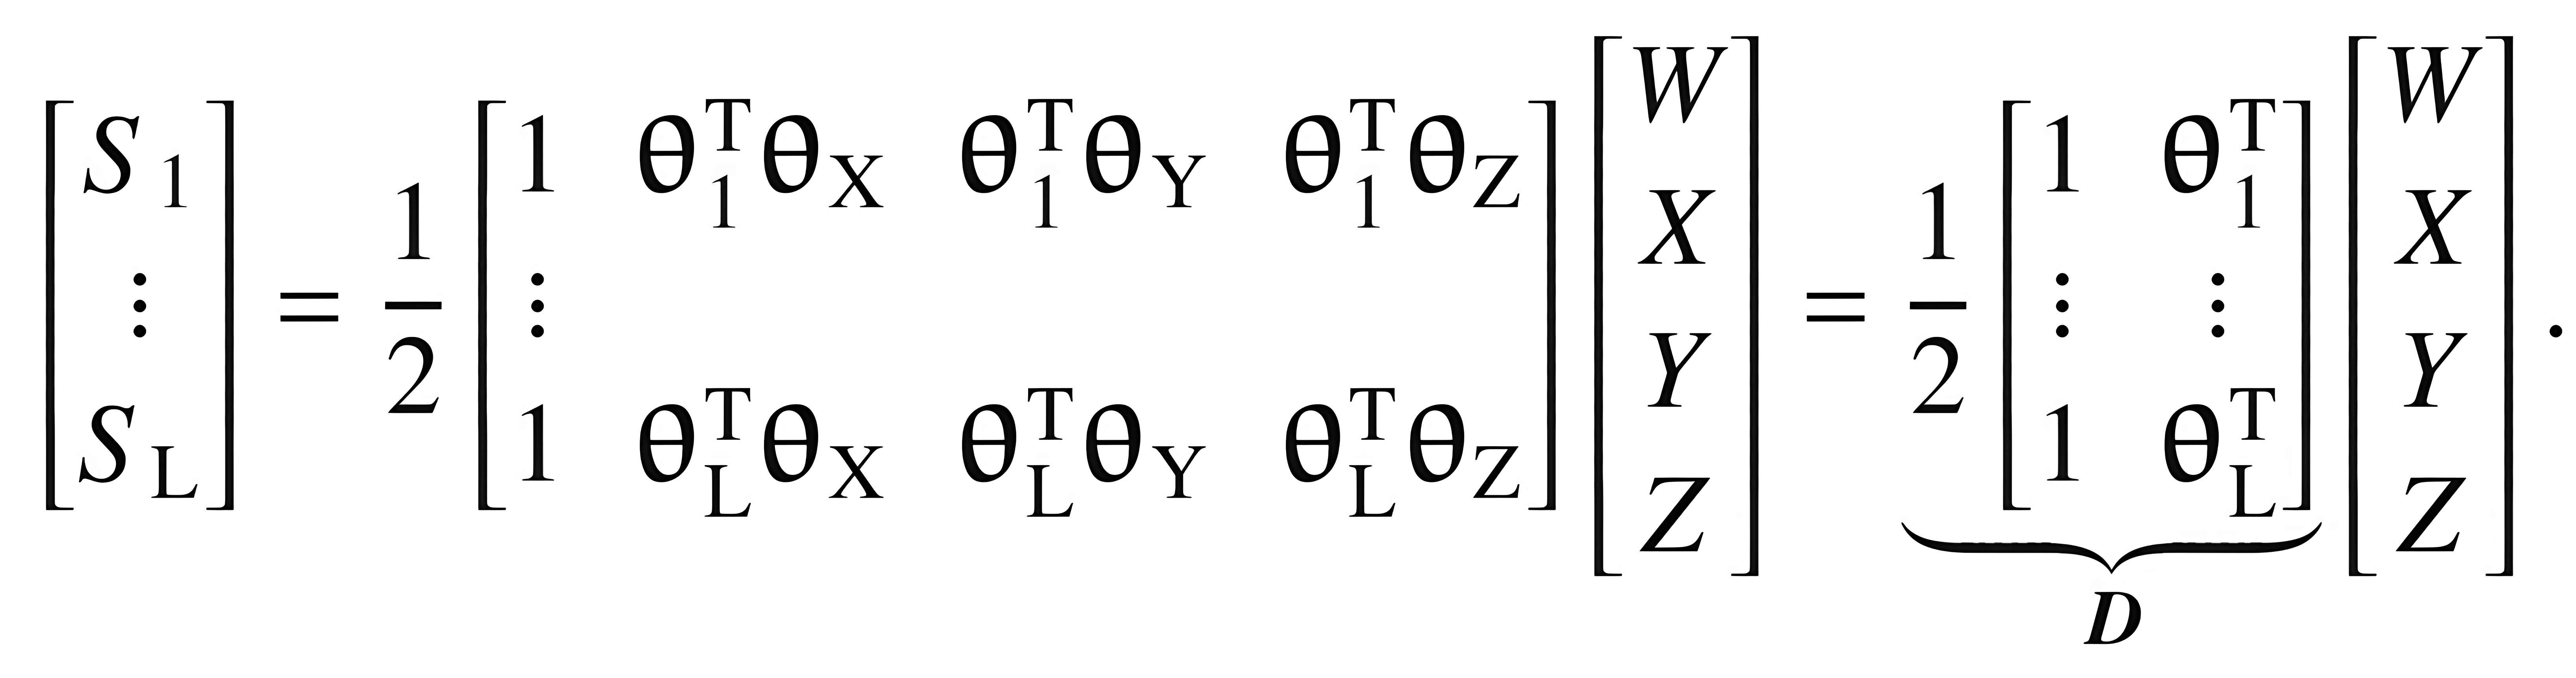
\includegraphics[width=0.7\textwidth]{images/spatial_audio/3d_sampling_decoder_equation.png}
    \caption{Decoding first order ambisonics using a sampling decoder.
        Image sourced from \cite{ambisonics_practical_theory}.
        \label{fig:3d_sampling_decoder_equation}}
\end{figure}

The presented decoder is called a ``sampling decoder" - ambisonic playback using such a decoder is ``comparable
to recording each signal with a virtual first-order cardioid microphone aligned with the loudspeaker's
direction $\Theta_l$". \cite{ambisonics_practical_theory} It is important to note that the speakers need to be uniformly spaced 
so the loudness of the resulting sound is not affected by the directional 
composition of the ambisonics signal
(so sounds coming from specific directions are not perceived as louder than sounds coming from elsewhere). 
An example of a 2D speaker array consisting of uniformly spaced speakers can be seen in figure \ref{fig:speaker_array}.

\begin{figure}
    \centering
    \includegraphics[height=20em]{images/spatial_audio/speaker_array.png}
    \caption{A 2D (horizontal plane) surround speaker array. Image courtesy of the author. \label{fig:speaker_array}}
\end{figure}

\subsection{Decoding to loudspeakers}

The ambisonics panning function $g(\theta)$ 
that yields the power of the signal for a given direction $\theta$ is continuous,
but in case of loudspeaker playback, the sound field must be recreated using a discrete number of point-sources. 
(See \cite{ambisonics_practical_theory} for the definition of $g(\theta)$ and a detailed dive into the math behind ambisonics.)
Only special arrangements of loudspeakers permit direct sampling without introducing undesired
direction-dependant gain variations (as described for first order ambisonics in the previous subsection). 
These so-called \emph{t-designs} are arrangements of speakers where the distance and direction between 
all neighbouring speakers are constant. $t \geq 2N + 1$ loudspeakers 
are required for optimal reproduction of ambisonics of order $N$. \cite{ambisonics_practical_theory}\cite{zotter_all_round_panning_and_decoding}

\paragraph*{Vector Based Amplitude Panning}

To describe some of the more advanced ambisonic decoding techniques, let's first introduce Vector Base Amplitude Panning (VBAP).
First described by Pulkki in 1997 in \cite{pulkki_dsp_tool_vbap_1996} and then in \cite{pulkki_vbap_1997},
VBAP provides a mathematical framework for selecting which loudspeakers from a 2D/3D 
surround arrangement should be activated and with what gains, to reproduce a virtual sound source at a specific direction.

In the simplest example of stereophonic amplitude panning (two speakers positioned in front of the listener),
Pulkki treats the loudspeaker direction vectors as a vector base.
A direction vector for a virtual sound source at an arbitrary point on the arc enclosed by the two loudspeakers
can be calculated as a linear combination of the two basis vectors. The coordinates of the sound source direction vector in that vector space 
are then interpreted as the gain values for each loudspeaker. 
This system is then extended to horizontal arrangements of more than 2 loudspeakers by always activating 
just 2 loudspeakers - the ones that form the arc on which the virtual sound source lies at that moment. 
As Pulkki states, utilising just two loudspeakers at a given time might seem wasteful, but this approach increases 
localisation accuracy. 

The 2D case is then generalised to 3D by utilising triplets of loudspeakers instead of pairs. 
An approach identical to the 2D case is used for arrays of more than 3 speakers.
Picking the correct speaker triplet to activate can however pose a problem in cases 
where the speaker arrangement allows for ambiguous triplet selection and some other situations.
Due to this, VBAP does favour specific speaker arrangements, but it is still a flexible approach 
that can be used in a variety of situations.
\cite{pulkki_vbap_1997}\cite{ambisonics_practical_theory}

\paragraph*{All-Round Ambisonic Decoding (AllRAD)}

The AllRAD approach presented in ``All-Round Ambisonic Panning and Decoding" 
by Franz Zotter and Matthias Frank \cite{zotter_all_round_panning_and_decoding}
combines VBAP and sampling decoders, as described in previous sections, 
to achieve a lower direction-dependant loudness variation and good spatial resolution
while also providing better results on irregular loudspeaker arrangements.

The idea behind AllRAD is first decoding (sampling) the ambisonic signal to a set of virtual speakers 
arranged in a $t$-design, and then using these signals as virtual sources for 
a slightly modified version of VBAP. Decoding to a regular arrangement of virtual loudspeakers
has the advantage of low directional gain variations and good sound localisation, while VBAP
makes this approach usable with real-life non-ideal speaker arrangements
(higher order $t$-design speaker arrays are usually not very practical).

For playback on speaker hemispheres (which are more common than full spheres in practice due to several factors),
as with normal VBAP, one or more imaginary loudspeakers may be added at the bottom of the arrangement,
or at the average direction vector of the real loudspeakers. The signal from the imaginary 
loudspeaker(s) may either be discarded or equally distributed to the neighbouring loudspeakers. 
While this approach does not actually reproduce the direction of sounds coming from below correctly,
it helps avoid the inability to find a matching speaker triplet (which would make these sounds inaudible),
and preserves some of the audio content coming from below (especially for sounds close to the outer ring of the speaker hemisphere).
A similar approach can of course be used for other speaker arrangements where there is no speakers in certain parts of the sphere.
\cite{ambisonic_decoders_slides_stanford}\cite{ambisonics_practical_theory}

I should note that while AllRAD is one of the most flexible and practical solutions available today,
there are multiple other decoding approaches. Overviews of the other approaches can be found in
\cite{ambisonics_practical_theory}, \cite{frank_and_franz_producing_in_ambisonics} and \cite{ambisonic_decoders_slides_stanford}.

\subsection{Decoding to headphones}

Since human listeners can detect directivity cues with just two ears, it stands to reason, that with the right 
technology, 360\degree{} sound can be reproduced on headphones just as well, if not better, than on loudspeaker arrays.
To achieve this, it is required that the main psychoacoustic cues used by humans (as described in section \ref{subsection:spatial_hearing})
are correctly reproduced. Ideally, interaural difference cues
and changes to the frequency composition of the sound induced by the listener's
head and ears need to be accounted for.

\begin{figure}[!ht]
    \centering
    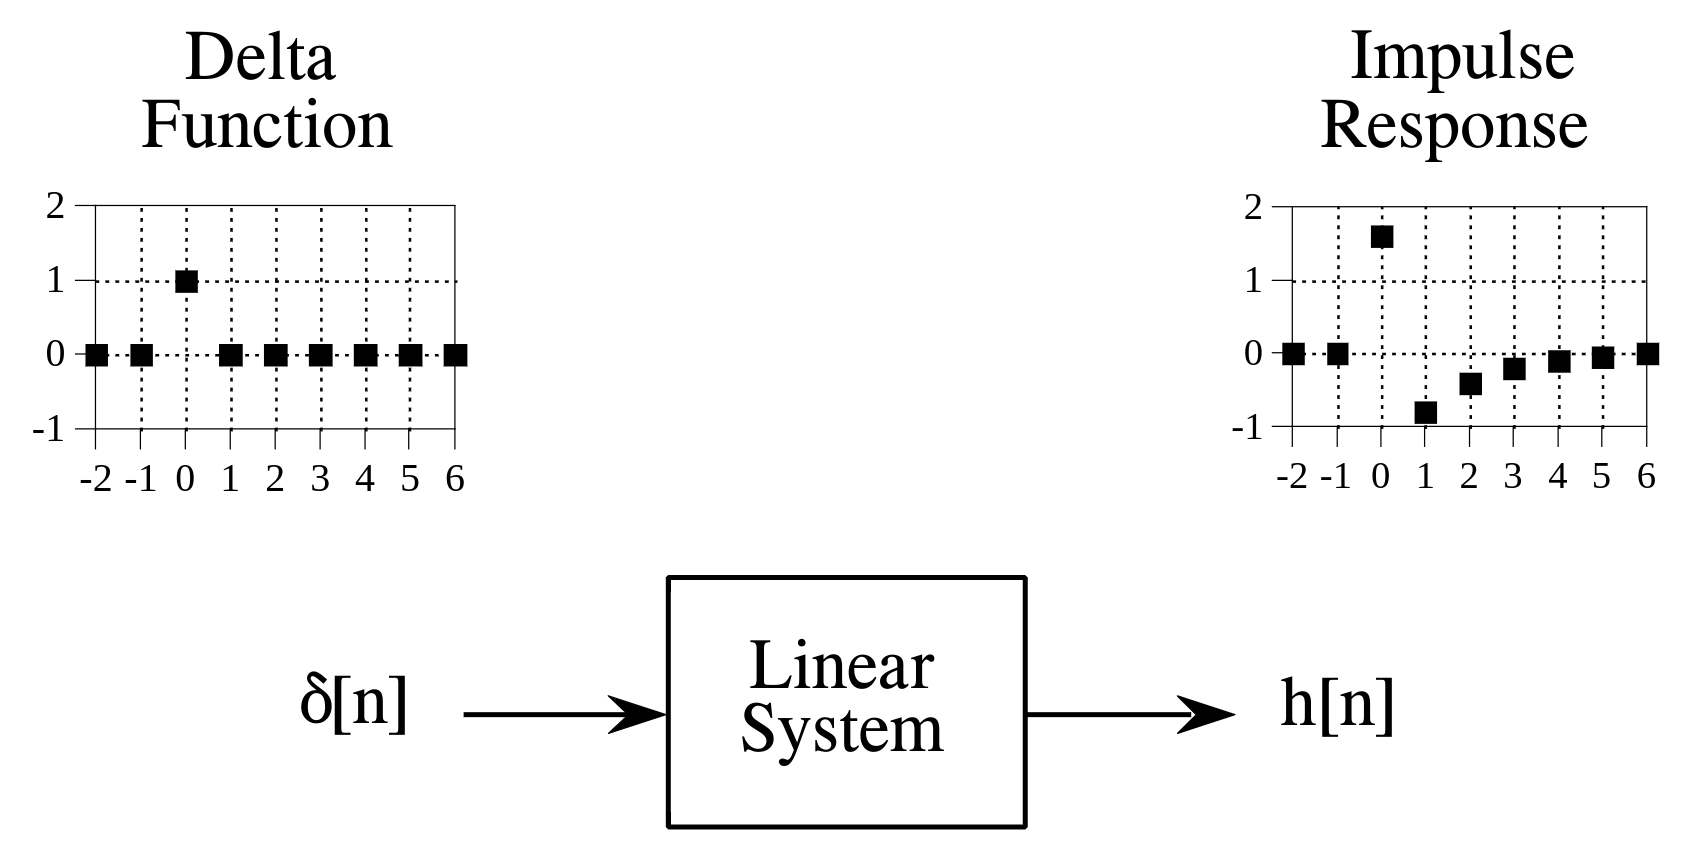
\includegraphics[height=14em]{images/spatial_audio/impulse_response.png}
    \caption{Definition of a delta function and an impulse response. $\delta[n]$ is used to identify the delta function. 
        The impulse response of a linear system is usually denoted by $h[n]$.
        Image sourced from \cite{dsp_book_convolution}. \label{fig:imp_resp_delta_func}}
\end{figure}

All of this can be captured using a so-called Head-related Impulse Response (HRIR).
First, let's figure out what an impulse response is in general. An impulse response is the output of a linear system when a delta function 
(unit impulse) is the input.
Considering a discrete signal ($N$ separate samples of a continuous signal),
a unit impulse is such a signal where the sample at position $0$ has a value of $1$, and all other samples have a value of $0$.
An important property of the delta function is that any signal can be represented as a combination of differently
shifted and scaled delta functions.\cite{dsp_book_convolution}
Figure \ref{fig:imp_resp_delta_func} provides a graphical definition of the delta function (unit impulse) and it's impulse response.
In the case of a HRIR, the impulse response represents how the listener's head and ears affect sound in a so-called free-field 
- an environment with no reflections or reverberations and thus no colouration of sound.\cite{fundamentals_of_binaural_technology}
Of course an ideal free-field environment can not be achieved in practice, but anechoic chambers get sufficiently close.

There are multiple methods and variations of methods of measuring a HRIR; a good in-depth overview can be found in \cite{hrtf_measurement_review}.
The core idea behind most of them is however the same - microphones are placed into the subject's ears, 
a specific sound (an excitation signal) is then played back (often multiple times)
over a loudspeaker located at a specific point in space, and then the impulse response 
of the system is calculated from the recorded audio.
Multiple measurements with the sound coming from different directions and sometimes distances have to be taken.
Often, especially in case of human subjects (as opposed to head models) it is desirable to move the position of the sound source instead of rotating the listener's head. 

In the time domain, the relation between the input and the output of the system is given by the following equation (\cite{dsp_book_convolution}):
\begin{equation}
    y(t) = x(t) * h(t) = \int_{-\infty}^{+\infty} x(\tau)h(t-\tau) d\tau,   
\end{equation}
where $x(t)$ is the input signal, $y(t)$ the output signal, $h(t)$ is the impulse response of the system, 
and $*$ denotes convolution. The same equation can be written for discrete signals as follows~(\cite{dsp_book_convolution}):
\begin{equation}
    y[n] = x[n] * h[n] = \sum_{j=0}^{N-1} h[j]h[n-j],
\end{equation}
for an N-point impulse response $h[n]$ with indexes spanning from $0$ to $N-1$.
Another term that the reader would surely encounter when researching ambisonic decoding to headphones,
and binaural audio in general is a head-related transfer function. A HRTF is nothing more than a HRIR 
in the frequency domain. \cite{fundamentals_of_binaural_technology} Once a HRIR is calculated, 
convolution can be utilised to calculate the response of the system to an arbitrary input signal.\cite{dsp_book_convolution}
Using HRTFs measured at different impulse directions, and utilising interpolation techniques, 
psychoacoustic cues for a sound coming from an arbitrary direction can be reproduced.\cite{hrtf_measurement_review}

Decoding ambisonic audio to headphones using HRTFs can be achieved by utilising virtual loudspeakers.
A decoder such as AllRAD is first used to produce a CBA signal set for some favourable arrangement of loudspeakers, such as a \emph{t}-design, to achieve low loudness variation and good localisation accuracy.
Each of the resulting virtual loudspeaker signals is then convolved with a HRTF measured at an appropriate direction.
Finally, the signals are added together to produce the final binaural mix. \cite{3d_ambisonic_based_binaural_reproduction}

It is worth mentioning that, as with most topics discussed thus far, there are many possible variations and improvements to the base approach. 
Some of them are discussed in \cite{ambisonics_practical_theory}.

\subsection{A comparison of personalised and generic HRTFs}

So-called personalised (or individualised) HRTFs are measured for a specific individual and thus
match how that person perceives sound in everyday life as closely as possible.
Generic HRTFs on the other hand are synthesized from large datasets of individual measurements 
with the aim to provide a good enough experience for most people.
Unsurprisingly, research shows that individualised HRTFs perform better than generic ones, with the main improvement being a reduction in front-to-back confusion.
\cite{localisation_nonindividualized_hrtfs}
However, non-personalised HRTFs show good enough performance in many cases, and are the more common choice in practice due to the 
cost and complexity of measuring individual HRTFs. 
Furthermore, with enough time, a listener's brain is able to adjust to a ``foreign" HRTF - experiments performed in 
\cite{adaptation_to_nonindividualised_hrtfs} show worse localization test performance by inexperienced subjects, 
than those that went through training (both simultaneously hearing a sound and seeing it's position, and trying to determine a sound's position with post-test feedback).
Trained subjects also showed better results when presented with sounds at positions different to the ones used during the training phase of the experiment.

Non-individualised HRTFs are already being widely used in interactive media, especially computer games. 
Sound localisation is important in first-person shooters and similar titles, and plays an enormous role in increasing immersion in VR. 
HRTFs are employed in Overwatch, Counter Strike: Global Offensive, Valorant, and many VR titles. 
There has also been some academic research into the usage of individualised and non-individualised HRTFs in video games.
While \cite{hrtfs_3d_shooter_game} concludes, that individualised HRTFs expectedly showed better localisation performance,
it is of note that the experiment results (Fig. \ref{fig:hrtf_3d_shooter_test_results}) showed a relatively similar horizontal localisation performance between 
(self-reported) experienced players when using non-individualised HRTFs and players using an individualised HRTF. 
This can realistically be attributed to ``expert" players having more experience with other FPS titles with HRTF-based spatial audio, 
as many of the most popular competitive titles do employ it.

\begin{figure}
    \centering
    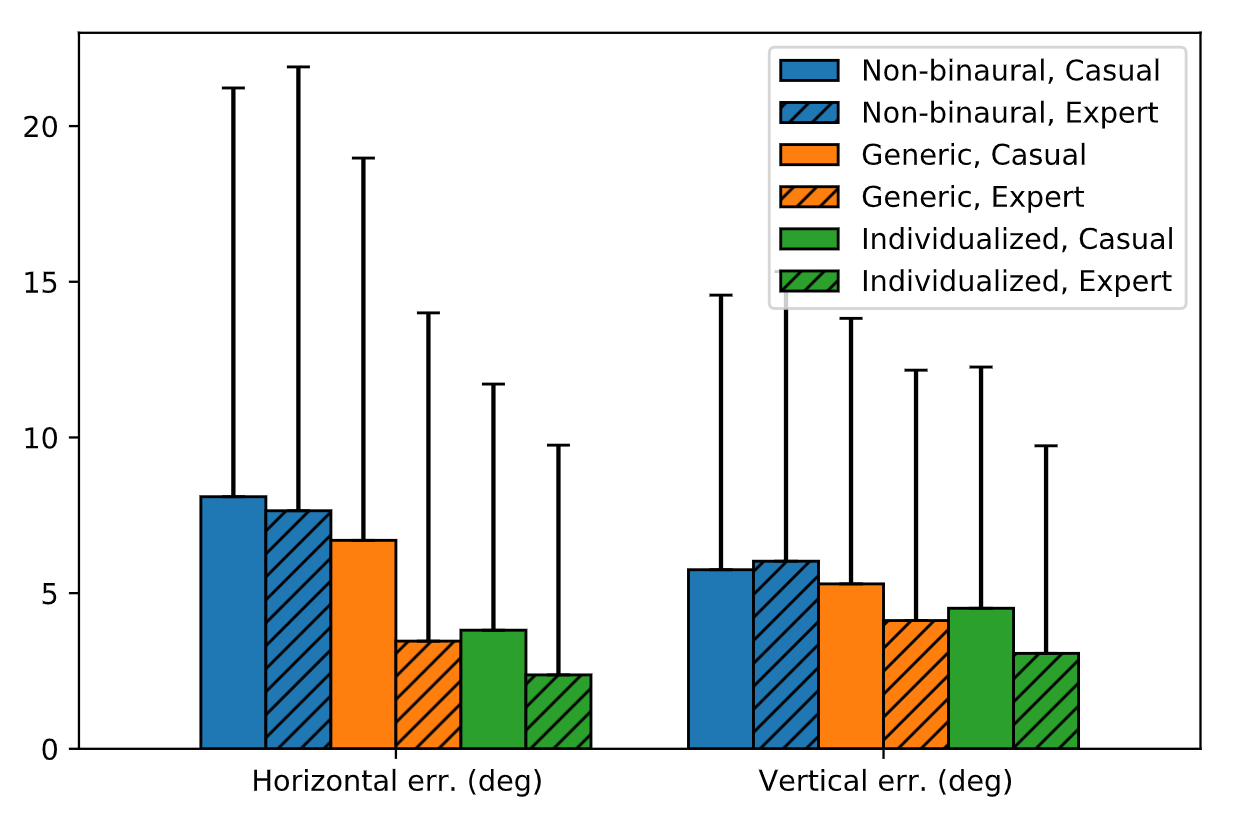
\includegraphics[width=0.5\textwidth]{images/spatial_audio/hrtf_fps_test_results.png}       
    \caption{Horizontal and vertical localization errors for expert (solid pattern) 
        and casual (hatched pattern) players. Image sourced from \cite{hrtfs_3d_shooter_game}.
        \label{fig:hrtf_3d_shooter_test_results}}
\end{figure}

Another study, that focused specifically on VR games \cite{generic_hrtfs_vr},
showed that sound localisation using generic HRTFs was improved with time, when the players were presented with 
matching visual and auditory stimuli. The improvements didn't occur when no visual stimulus accompanied the sound, 
or when the stimuli were not sufficiently synchronised. The experiments also showed that the improvements in 
localisation didn't transfer to different auditory stimuli (sounds with a significantly different spectral composition).
This however should not pose a problem in case of video games and other hand-crafted experiences,
as they tend to use a comparatively low number of individual sounds, especially 
if only sounds whose accurate localisation is important to the overall experience are taken into account.

%//TODO: mention applied binaural audio somewhere? (apple music spatial audio, etc)

% \cite{blumlein_patent}

\chapter{An overview of spatial audio production software}

\begin{chapterabstract}
    This chapter examines some of the spatial audio production tools
    publicly available at the time of writing and discusses their suitability
    for 360\degree{} video production.
\end{chapterabstract}

\section{DAW-based solutions}

Most tools for producing ambisonic audio come in the form of DAW plugins, most of them in the VST format\footnote{
    VST is a plugin format for digital audio workstations developed by Steinberg Media Technologies. \cite{vst_steinberg}
    While competing plugin formats exist, VST is multiplatform, and one of the most widely supported ones.
}.
They are usually released in the form of plugin suites, consisting of ambisonics encoders (panners) and decoders.

The encoder plugin takes an input (in most cases mono or stereo), computes the spherical harmonic coefficients, 
based on the current panning settings, and outputs an ambisonics representation with the sound placed at the desired direction relative to the listener.
An instance of the encoding plugin has to be placed on each channel that will be used in the final ambisonics mix, as can be seen in figure \ref{fig:encoders_routing}.
Recordings from microphone arrays, and other ambisonic audio can also easily be added to the final mix by simply adding the individual channels together.

\begin{figure}
\centering
    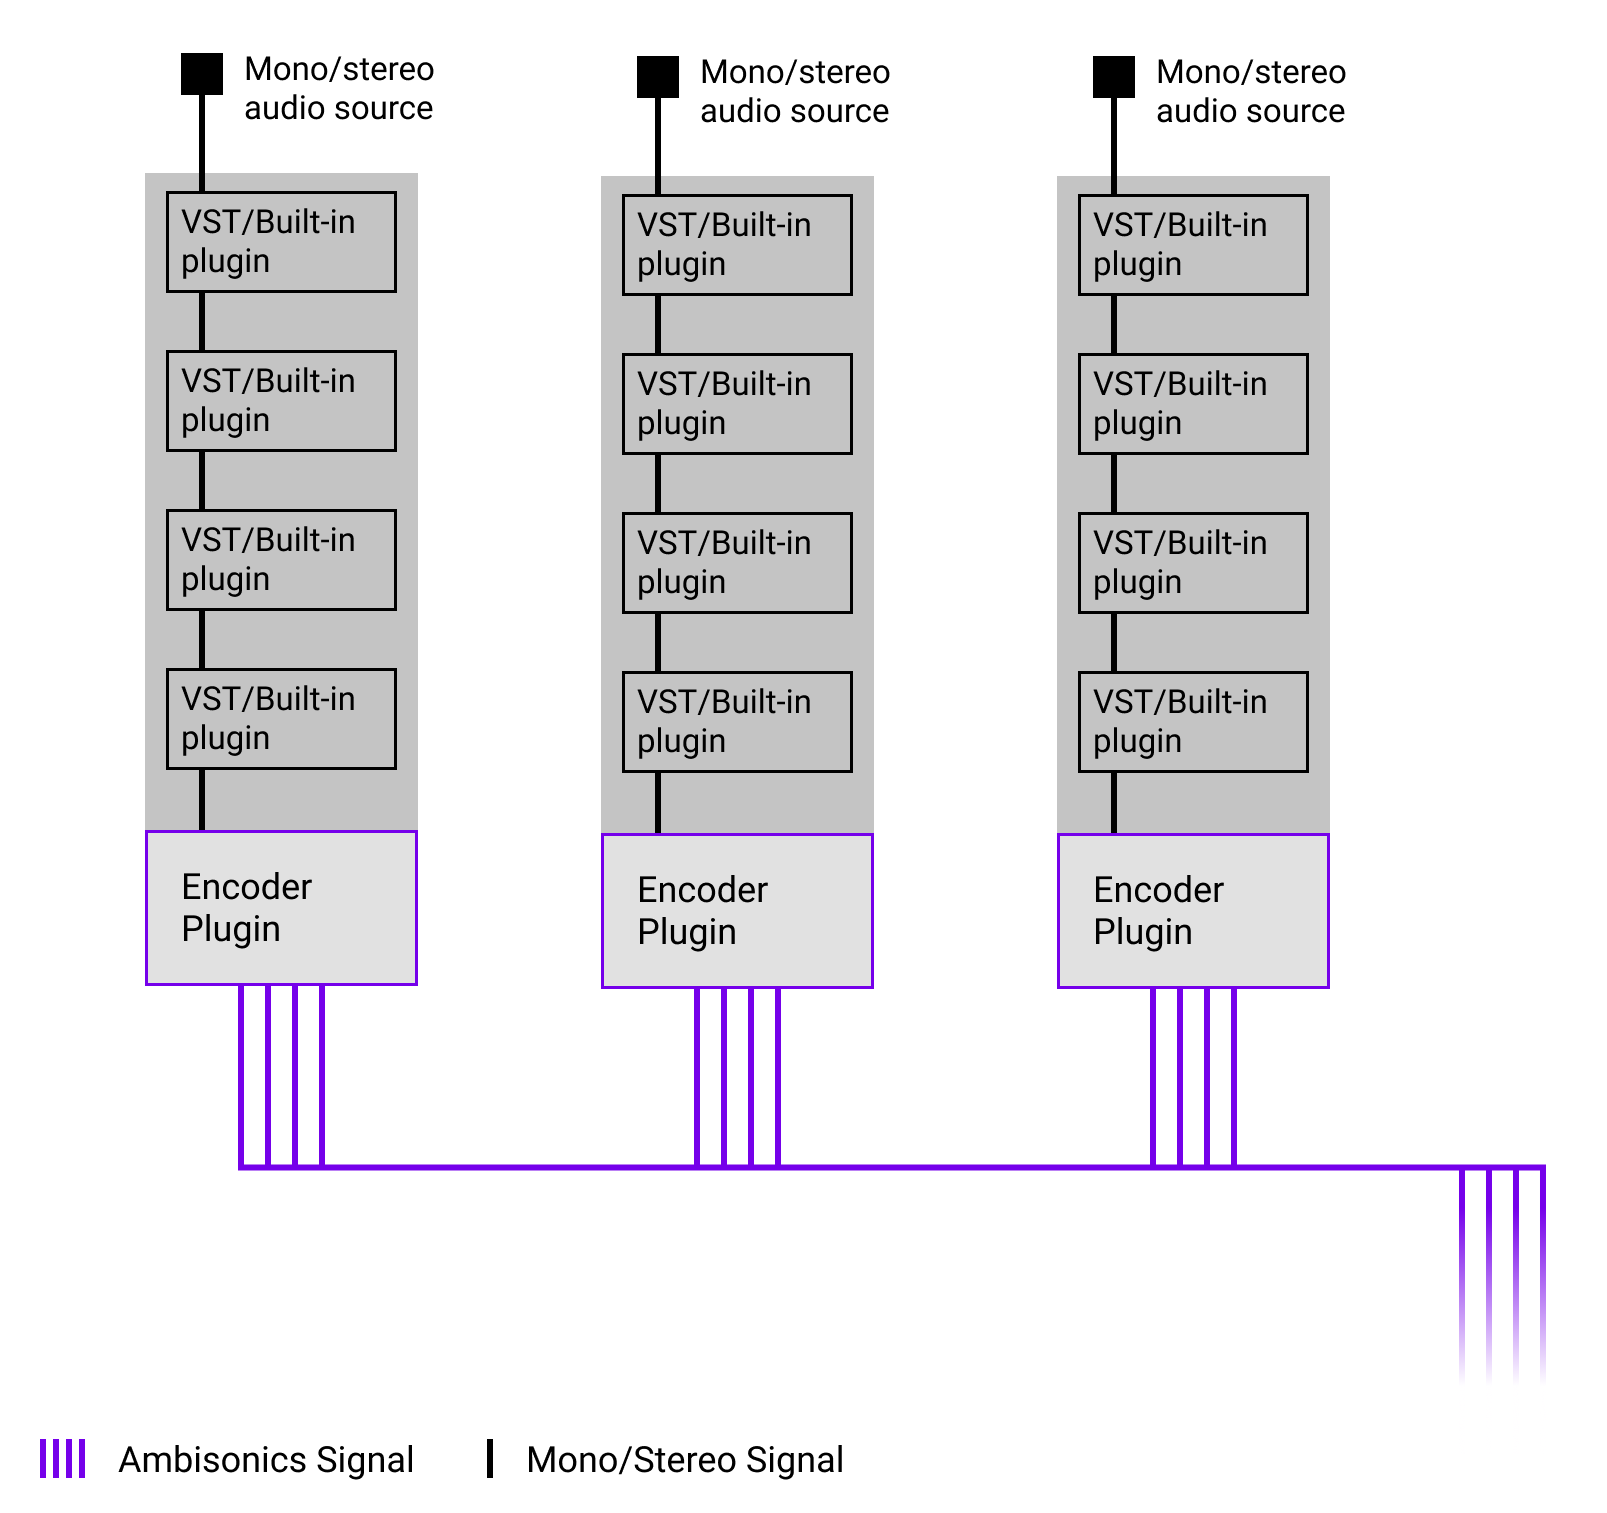
\includegraphics[height=32em]{images/daws_vsts/encoders_setup_cropped.png}       
    \caption{Ambisonic encoder plugins placed on individual channels. Image courtesy of the author. \label{fig:encoders_routing}}
\end{figure}

Using the encoder alone is enough to output an ambisonics mix, but in order for the mixing engineer to hear 
the results of his actions, or to output the mix in CBA format, the ambisonics representation has to be decoded back to channel-based audio.
For these purposes these plugin suites usually include a decoder plugin that converts the ambisonics signals into speaker
feeds for a surround setup, or into a stereo binaural representation using a personalized or generic HRTF.
The decoding plugin is usually placed on the master bus\footnote{A master bus is the final stage in audio processing. It combines the signals from all the individual channels (or tracks) in a DAW or a hardware mixing console.}
- figure \ref{fig:decoder_master}.

\begin{figure}
    \centering
    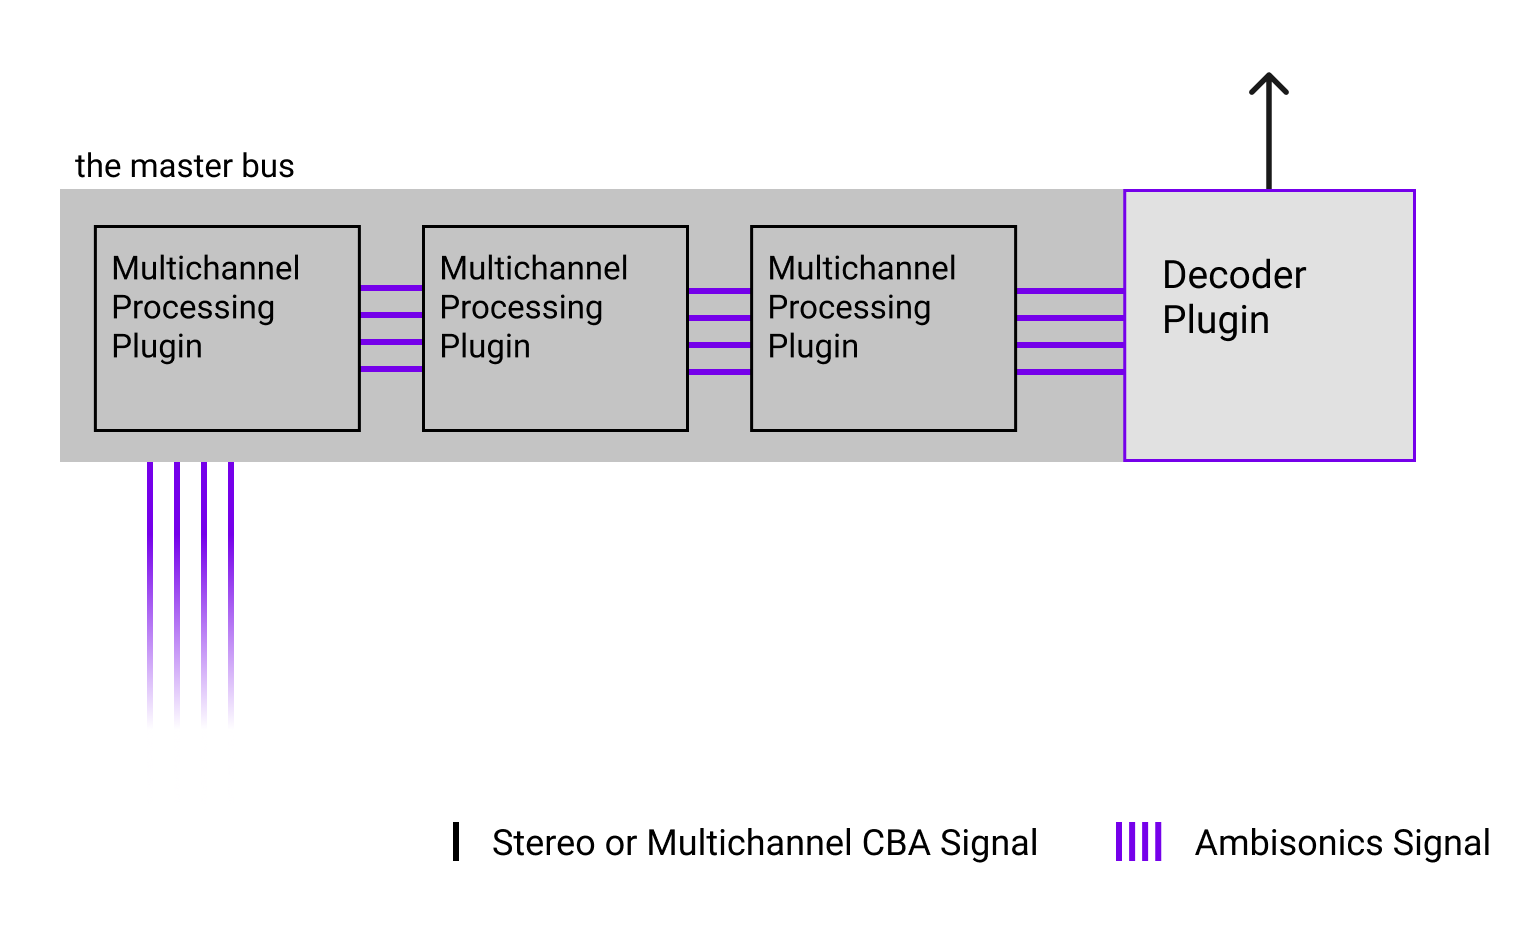
\includegraphics[height=19em]{images/daws_vsts/master_bus_setup_cropped.png}       
    \caption{A master bus with an ambisonics decoder plugin. Image courtesy of the author. \label{fig:decoder_master}}
\end{figure}

Because the plugin outputs multiple channels of audio, 
the digital audio workstation itself has to provide support for multichannel audio.
The maximum achievable ambisonics order is then limited by three factors - 
available computational power (for real time preview), the plugin itself, and the number of channels supported by 
the DAW. Fortunately, while not prevalent, multi-channel support is present is some of the 
popular digital audio workstations, such as Reaper \cite{reaper_manual} and Pro Tools \cite{protools_manual}; 
Steinberg's Cubase Pro even provides built-in ambisonics support in the form of encoder and decoder plugins, as well as general multi-channel capabilities \cite{cubase_ambisonics}.
Nuendo - another DAW from Steinberg, geared towards industry professionals, provides ambisonics support with advanced features
- their decoder, for example, supports head-tracking to synchronize the audio with head movement (Fig. \ref{fig:nuendo_screenshot}). 
Nuendo also has built-in integration with some game audio middleware systems
\footnote{Middleware systems are software that is integrated into a game engine to handle a specific subset of it's functionality, such as audio playback.}
(Wwise and ADX2), as well as features specific to VR audio
, including support for dearVR Spatial Connect - a virtual reality environment for spatial audio mixing,
which also provides positional data export to the Unity game engine.
\cite{nuendo_features}

\begin{figure}[!ht]
    \centering
    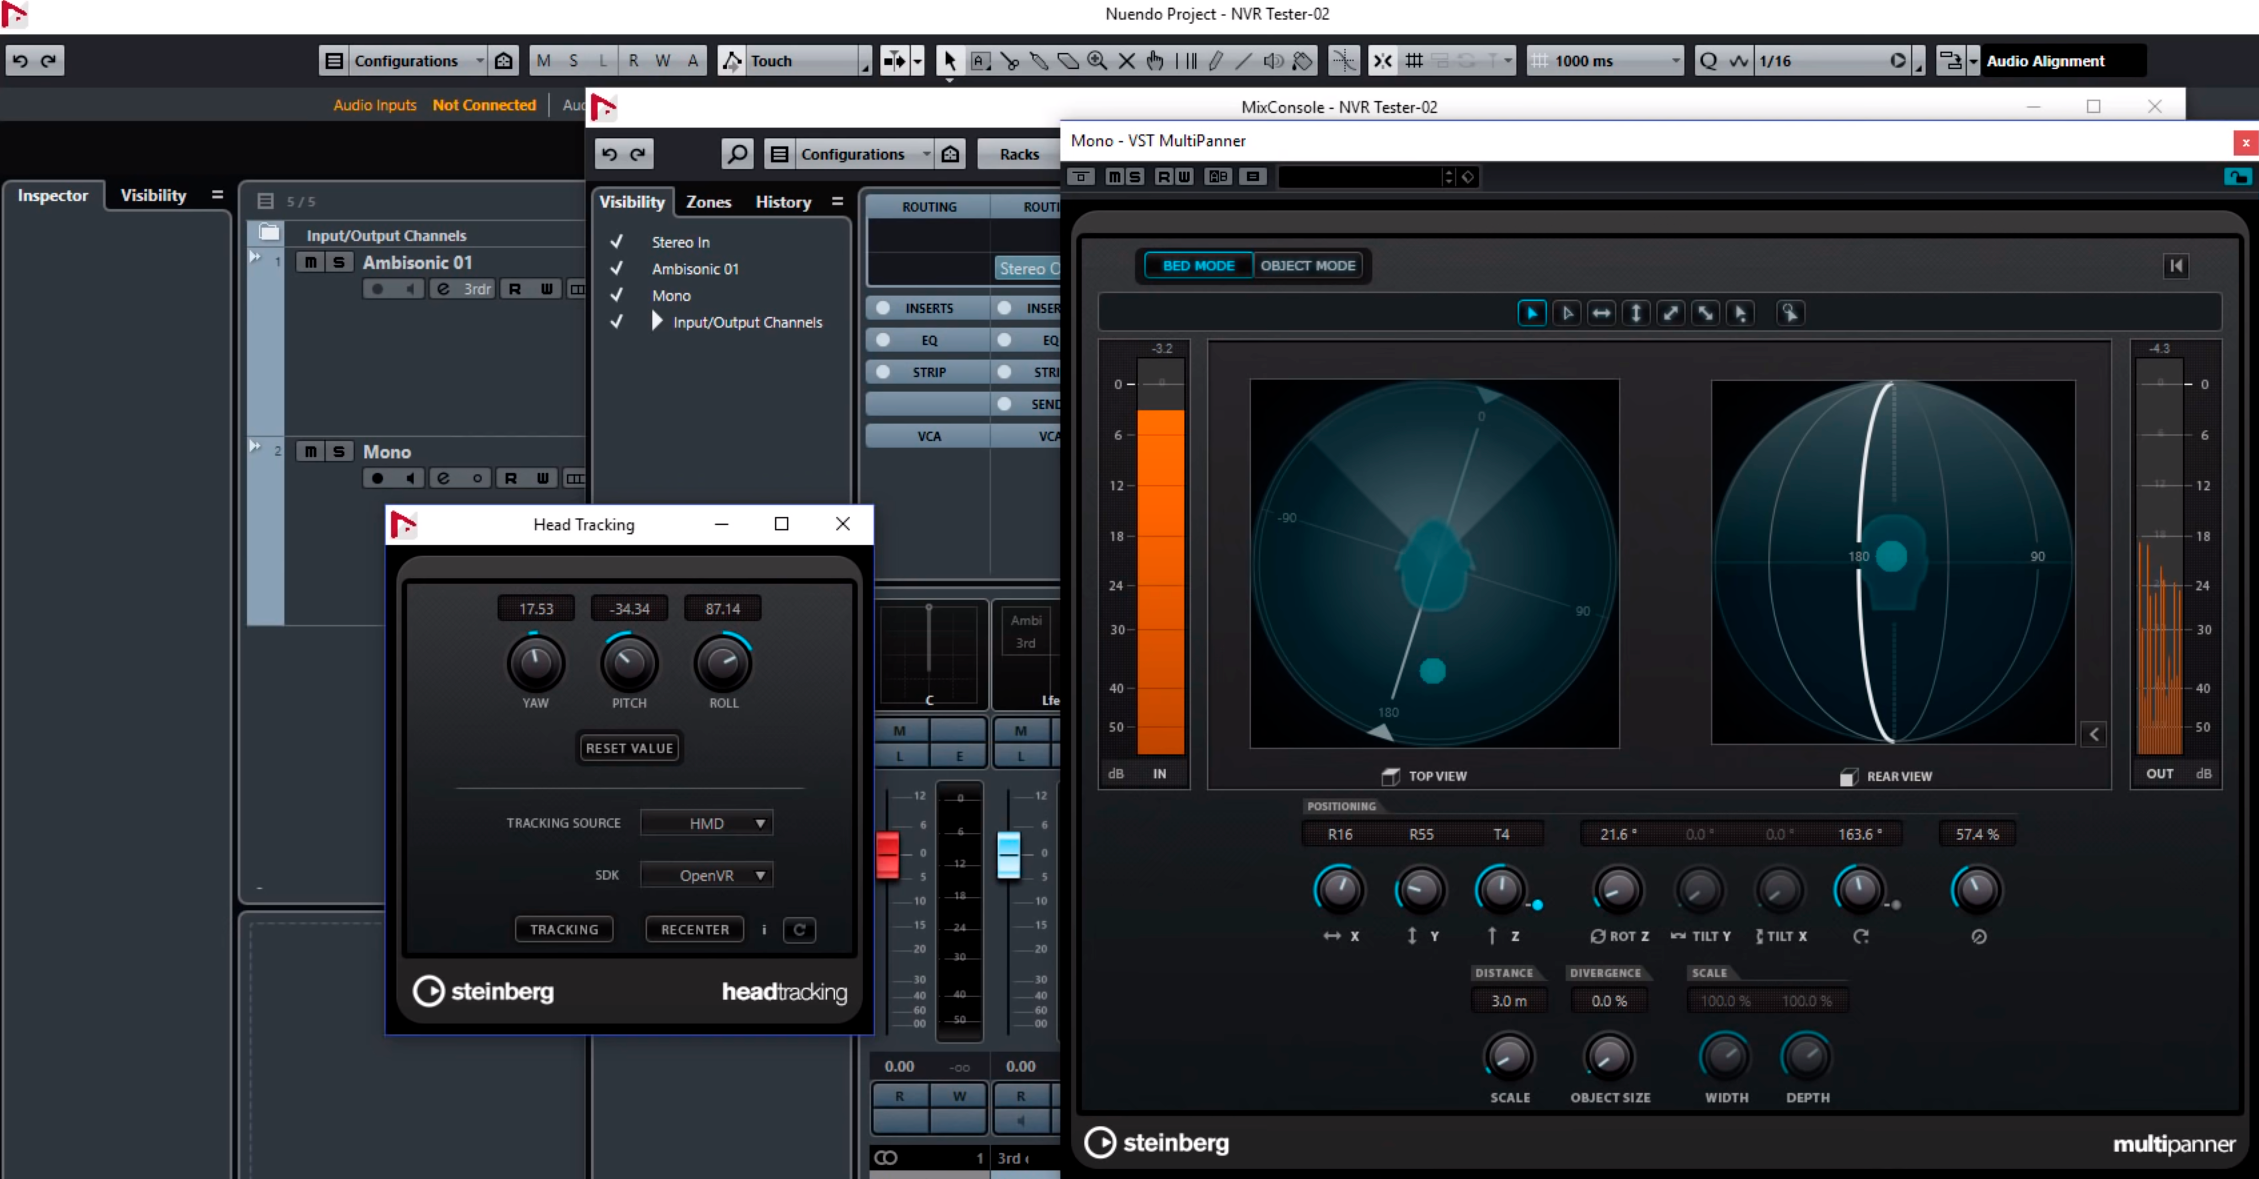
\includegraphics[width=\textwidth]{images/existing_solutions/nuendo_panner_and_head_tracking.png}       
    \caption{Head-tracking and spatial panning in Steinberg's Nuendo.
        Image sourced from \cite{nuendo_screenshot}.
        \label{fig:nuendo_screenshot}}
\end{figure}

Ambisonic plugin suites usually include multiple types of encoders and decoders. 
Various encoders can be used for encoding non-ambisonic content with different directivity patterns, 
e.g. planewave (sound emanating from a single direction) or omnidirectional,
as well as transforming recordings from various microphone arrangements into a standardised ambisonics representation.
Decoders usually differ in their output format - CBA for various speaker arrangements, binaural stereo, etc.

Listed below are some of the more fully featured ambisonics plugin suites (with a bias towards open source).
\begin{itemize}
    \item The Ambisonic Toolkit \cite{ambisonic_toolkit}
    \item ambiX \cite{ambiX}
    \item IEM Plug-in Suite \cite{iem_plugin_suite}
\end{itemize}

The DAW-based approach to spatial audio production provides a lot of flexibility,
especially if working in Reaper or another DAW with similar multichannel and routing capabilities.
The producer is able to use the in-DAW workflows they have grown accustomed to and can benefit
from the vast amount of available plugins. Plugins from different manufacturers, including ambisonic encoders, decoders, 
and spatial effects, can all be used in a single project.
This is approach is popular and flexible, but there is definitely still room for improvement, 
especially for more specialised workflows such as 360\degree{} video production.
One area for improvement is integration between the different software used throughout the production process.
Such functionality is absent from most DAWs, which is to be expected due to the relatively 
low number of users that would benefit from it.
Fortunately, in many cases, such workflows can be improved by plugin developers.

\section{Game Engines}

While digital audio workstations are the obvious choice when it comes to producing any form of audio content, 
including ambisonics, in some cases, other approaches may be more sensible. 
The visual fidelity of modern game engines is already on such a high level, that they can be used for
3D productions. Their object-based audio systems also provide extensive 
functionality including mixing and real time audio processing. \cite{unreal_doc_audio}\cite{unity_manual_audio}
Theoretically, this could allow them to be used as an all-in-one 360\degree{} video production tool.
Unfortunately, in reality, using game engines for 360\degree{} video production might not be a good choice.
Neither of the two most popular commercially available 
game engines provide reliable solutions for exporting 360\degree{} video and audio.

Unreal Engine does come with the ability to export 360\degree{} video out of the box, but only as a series of still
images, and thus without audio. Exporting ambisonics is not supported in any way at the time of writing, 
although workarounds, converting a CBA mix from unreal to ambisonics, can be devised (but quality loss would be inevitable in that case). \cite{unreal_360_export}
Unity doesn't have built-in support for exporting 360\degree{} video or audio, but a third-party solution 
is available.
The "VR Panorama 360 PRO Renderer" tool's Unity Asset Store page \cite{unity_360_export} does claim to support rendering 
360\degree{} video, as well as ambisonics audio ``for YouTube''. But the quality of the implementation and integration with Unity is not guaranteed,
this being a third-party product.

Being able to use a single piece of software
for both the visual and the audio aspects of production is certainly attractive.
Unfortunately, the major commercially available game engines are not currently viable for 360\degree{} video production.
Their feature-set, however, despite being intended for a different use case, 
already provides a great foundation that can be built upon 
by adding some 360\degree{} video specific features.
With the popularisation of spherical video and VR gaming, it is possible that
360\degree{} gameplay demos and game trailers will become more common, and such features will 
be added as demand increases.

\section{3D software}

Studying the manuals for multiple widely adopted 3D software packages
\footnote{Blender, Autodesk Maya, Maxon Cinema 4D, Autodesk 3ds Max, and SideFX Houdini.}
leads to an unsurprising finding - most lack audio features in general, let alone SBA export capabilities.

Both Autodesk's offerings - Maya and 3ds Max provide some degree of audio support, 
but these features are limited and not usable in a spatial audio context. 
Maya's audio support is intended purely for synchronising animation to sound. \cite{maya_manual_audio}
3ds Max does provide a more fully featured audio editing system, but it's limited to arranging pre-rendered CBA clips, 
and is incapable of spatial audio encoding in any form. \cite{3dsmax_manual_audio}

Blender on the other hand does include a spatial sound system.
The user can place speaker objects, representing individual sound sources at arbitrary positions in the 3D scene.
The software allows to choose between several distance fall-off models, adjust the direction in which the sound is emitted 
from each individual speaker object, and even includes doppler effect simulation.~\cite{blender_manual_audio}
The unfortunate part is, that the current version of Blender (at the time of writing - 3.1) only supports exporting stereo.
It is not documented anywhere which technique is used to render this stereo output, but,
based on my listening test\footnote{
    I placed a speaker object directly above a camera moving on the vertical axis, and listened to the result to
    check if there was any height information present.
}, it is not binaural stereo. Interestingly, earlier versions of Blender
(at least up until v2.79\footnote{
    Downloading and launching the aforementioned version of the software confirmed that the feature is present.
})
did include the ability to export 5.1 and 7.1 surround audio, but it has later been removed.
Overall, Blender itself
can also be deemed unusable for spatial audio production.
A Blender add-on which implements OBA export will be mentioned in the next subsection.

There is however an outlier, both in terms of spatial audio support, 
and in terms of the software's general purpose - SideFX's Houdini.
A software with a target audience intersecting those of the previously mentioned programs only to a lesser extent, 
Houdini takes a completely procedural approach to 3D and includes advanced simulation capabilities.
Audio simulation capabilities are also present, and ``simulation" is truly the correct word to use here.
Houdini's spatial audio system supports distance fall-off, doppler effect, and even obstacle interference,
including per-obstacle customisation of transmission and absorption levels for different frequencies.~\cite{houdini_spatial_chop}\cite{houdini_acoustic_chop}
As in Blender, sound objects with customisable emission direction can be placed in the 3D scene. \cite{houdini_sound_object}
The sound can then be ``captured'' by an arbitrary amount of virtual microphone objects \cite{houdini_microphone_object}, effectively allowing
to record audio using microphone setups analogous to those used in the real-world, which makes ambisonics and CBA recordings possible.
While I could not find any examples of spatial audio rendered using Houdini, and thus can not assess the quality of the output,
the capabilities of this solution seem vast.
Houdini, however, is not an audio production environment. Using it's spatial audio system, as with it's other aspects,
requires much more specialised knowledge than using other approaches, such as DAWs and game engines.

\section{Other solutions}

This section includes some interesting solutions that didn't fall into any of the above categories 
and don't have alternatives that would warrant adding a separate subsection. 
% Some of them are not strictly related to 360\degree{} video production, but I still felt their 
% inclusion would benefit the reader in terms of providing a broader overview of the spatial audio field.

\paragraph*{IRCAM Panoramix}
Designed and developed at IRCAM
(French: Institut de recherche et coordination acoustique/musique, English: Institute for Research and Coordination in Acoustics/Music), 
Panoramix is a post-production and mixing workstation for 3D-audio content. 
It aims to provide a 
``comprehensive environment for mixing, reverberating, and spatializing sound materials from different microphone systems:
surround microphone trees, spot microphones, ambient miking, Higher Order Ambisonics capture.''
(\cite{panoramix_conference_paper})
It is not meant to replace a digital audio workstation, but rather work in conjunction with one, 
aiding in the mixing stage of the production workflow. 
The design is inspired by hardware mixing decks with each track represented by a vertical strip. 
There are various types of input tracks, accommodating different input signal types, e.g. mono, ambisonic, different microphone arrangements.
It also includes various other tools useful in spatial mixing and mastering, such as a reverberation engine, 
as well as the usual mixing instruments - an equaliser and a compressor/expander. 
A concise feature list can be found in \cite{panoramix_ircam_website}; a conference paper (\cite{panoramix_conference_paper}),
that delves deeper into the motivation behind creating the software
and the design decisions made in the process might also be of interest to the reader.

\paragraph*{The ``soundobjects'' Blender add-on}
Created by Jamie Hardt (@luvcapra on GitHub), ``soundobjects'' is a Blender add-on
that allows export of OBA in the ADM Broadcast WAV format. (See \cite{dolby_adm_spec} for the format specification.)
It provides Blender operators that allow to import WAV audio files, add speaker objects to existing objects in the scene, assign audio files to them, 
and export a file in the ADM Broadcast-WAV format where each audio object corresponds to a Blender speaker object in the scene.
The resulting file contains a sound object for each of the speaker objects in the blender scene.

Unfortunately, it seems this project is no longer being developed or maintained. 
The last commit in the project's GitHub repository (\cite{soundobjects_addon_repo}) adds a note 
about changes in ProTools that result in the inability to import WAV files produced by the add-on.
Despite this, the project is still an interesting tool, and, with interest from the open source community, 
could be revitalised and improved.

% \section{Summary}
% Of all the approaches presented in this sections, the ecosystem around producing ambisonics using 
% digital audio workstations seems to be the most evolved. 
% Since manipulation and creation of 
% audio content is the sole purpose of DAWs, it is unsurprising that the software is being adapted for spatial audio.
% While other approaches should still be considered depending on the task at hand,
% the versatility and extensibility provided by a DAW-based spatial audio production workflow 
% makes it the clear winner for producing
% // TODO: maybe add summary section if there's time

